\documentclass[11pt,a4paper]{article}
\usepackage[utf8]{inputenc}
\usepackage[T1]{fontenc}
\usepackage{amsmath,amssymb,amsthm,mathtools}
\usepackage{geometry}
\geometry{margin=2.2cm}
\usepackage{booktabs,longtable,array}
\usepackage{xcolor}
\usepackage{enumitem}
\usepackage{lmodern}
\usepackage{microtype}
\usepackage{tikz}
\usepackage{hyperref}
\hypersetup{
    colorlinks=true,
    linkcolor=blue!70!black,
    citecolor=red!70!black,
    urlcolor=blue!70!black,
    pdftitle={Unconditional Arithmetic Reductions, Exact Cotangent Reciprocity, and Lean 4 Formal Verification for the Classical and Nyman-Beurling Theory of the Riemann Zeta Function},
    pdfauthor={Qamar Munawer}
}

\newtheorem{theorem}{Theorem}[section]
\newtheorem{lemma}[theorem]{Lemma}
\newtheorem{proposition}[theorem]{Proposition}
\newtheorem{corollary}[theorem]{Corollary}
\theoremstyle{definition}
\newtheorem{definition}[theorem]{Definition}
\newtheorem{remark}[theorem]{Remark}

\newcommand{\R}{\mathbb{R}}
\newcommand{\C}{\mathbb{C}}
\newcommand{\N}{\mathbb{N}}
\newcommand{\Z}{\mathbb{Z}}
\newcommand{\Q}{\mathbb{Q}}
\newcommand{\Acal}{\mathcal{A}}
\newcommand{\Pcal}{\mathcal{P}}

\title{\textbf{Unconditional Arithmetic Reductions, Exact Cotangent Reciprocity, and Lean~4 Formal Verification for the Classical and Nyman--Beurling Theory of the Riemann Zeta Function}}

\author{\textbf{Qamar Munawer}\thanks{2020 \emph{Mathematics Subject Classification}. Primary 11M26; Secondary 46E20, 68V20. Formal Lean~4.35 verification artifacts are archived at \texttt{https://doi.org/10.5281/zenodo.24357255} (prev \texttt{10.5281/zenodo.24353918}; Concept DOI \texttt{10.5281/zenodo.24150107}) alongside Paper~M at \texttt{https://doi.org/10.5281/zenodo.24357107}.}\\[0.25em]
\small Brandenburg University of Technology Cottbus--Senftenberg}

\date{November 19, 2026}

\begin{document}
\linespread{1.12}\selectfont
\emergencystretch=3em

\maketitle

\begin{abstract}
The classical theory of the Riemann zeta function $\zeta(s)$ and the Hilbert-space Nyman--Beurling--B\'aez--Duarte program share a remarkably tight algebraic backbone. Unconditionally, de~la~Vall\'ee~Poussin's classical trigonometric barrier secures a zero-free strip $\sigma > 1 - c/\ln|t|$ while Hardy's theta--Mellin moment argument forces infinitely many zeros onto $\operatorname{Re}(s) = 1/2$; conditionally, Littlewood's remainder bound, von~Koch's Chebyshev $\psi$ estimate, reciprocal zeta holomorphy, and Titchmarsh's bidirectional Mellin identity link zero-freeness in $\operatorname{Re}(s) > 1/2$ to $L^2(0,1)$ approximation of~$1$ by fractional parts $\rho_k(x) = \{1/(kx)\}$. Restricting finite linear combinations $\sum_{k=1}^N c_k \rho_k$ to the B\'aez--Duarte affine manifold ($D_1 = 0, D_0 = 2$) cancels the continuous slope $(\tfrac{1}{x} - n) D_1$ inside every harmonic interval $n \le \tfrac{1}{x} < n+1$, collapsing the continuous residual onto both the integer floor sum $1 + \sum_{k=1}^N c_k \lfloor n/k \rfloor$ and the modular sum $A_c(n) = 1 - \sum_{k=1}^N c_k \{n/k\}$, forcing exact periodicity $A_c(n+L)=A_c(n)$ for any common multiple $L$ of $1,\dots,N$ with palindromic antisymmetry $A_c(L - 1 - m) = -A_c(m)$ and zero period mean, while annihilating Euler's constant $\gamma$, $\ln(2\pi)$, and Vasyunin's smooth logarithmic kernel $G_{\mathrm{smooth}}$ in $L^2(0,1)$. Expanding in $4$-point cumulative wavelet dipoles $v^{(m)}$ isolates an $N$-independent Gram matrix $\widetilde{G}_{a,b}$ whose Rank-$2$ linear boundary drift cancels identically against the two-point anchor $(-2, 4)$ and reveals a pure plaque form $\mathcal{P}_N$. Locking the pole coefficient $c_1 = -1$ both annihilates the continuous residual identically on the entire top half $x \in (1/2, 1]$ and induces an exact unit partition ($\sum_{k=2}^N c_k/k = 1$, $\sum_{m=1}^{N-2}\alpha_m = 1$) absorbing constant target energy and linear drive symmetrically into the homogeneous unit-defect kernel $\mathcal{M}_{ab}$. Exact closed-form evaluations at $N = 3, 4, 5, 6$ establish rational $\sqrt{3}$ cancellation at $\tfrac{31}{108}\pi$, pentagonal $(\Z/5\Z)^\times$ reciprocity, and $N=6$ decoupling, while universal periodicity and reflection symmetry of Vasyunin sums prove octave vanishing $K_{\mathrm{cot}}(k,2k) = 0$, all-$m$ superdiagonal dipole orthogonality $\widetilde{G}_{m,m+1} = 0$, 1D plaque row-sum telescoping to $\pi V(N,2)$, and a symmetric Graph-Laplacian simplex decomposition. All analytic and algebraic theorems are verified in Lean~4.35 alongside $85$-digit and $512$-bit numerical diagnostics across $N \le 750$.
\end{abstract}

\noindent\textbf{Keywords:} Riemann Hypothesis, Nyman--Beurling criterion, Vasyunin cotangent sums, cumulative wavelet dipoles, Dirichlet anchoring, Graph-Laplacian simplex, Lean~4.

\tableofcontents
\clearpage

\section{Mathematical Scope and Formal Architecture}\label{sec:intro}

Establishing a rigid separation between unconditionally proved theorems, conditional equivalences for the Riemann Hypothesis (RH), and certified finite-horizon numerical computations is essential in analytic number theory~\cite{Riemann1859,Titchmarsh1986}. Every theorem treated below falls cleanly into one of three categories:
\begin{enumerate}[leftmargin=1.8em,itemsep=2pt]
\item \textbf{Unconditional Analytic and Algebraic Theorems:} Classical zero-free region and critical-line results (de~la~Vall\'ee~Poussin~\cite{deLaValleePoussin1899}, Hardy~\cite{Hardy1914}, functional derivative antisymmetry $\Lambda'(1/2)=0$, and prime--composite Dirichlet series splitting in $\operatorname{Re}(s)>1$), paired with exact all-$N$ algebraic reductions, $N=3,4,5,6$ radical reciprocity identities, all-$m$ superdiagonal dipole orthogonality, and 1D/2D discrete Abel telescoping on the B\'aez--Duarte manifold $\mathcal{A}_N$.
\item \textbf{Conditional RH Equivalences:} Bidirectional analytic links between the Riemann Hypothesis and reciprocal zeta holomorphy, Littlewood's $O(x^{1/2+\varepsilon})$ Mertens criterion~\cite{Littlewood1912}, von~Koch's Chebyshev $\psi$ remainder~\cite{vonKoch1901}, bidirectional Mellin Nyman--Beurling approximation~\cite{Nyman1950,Beurling1955,BalazardSaiasYor1999}, and the pure plaque / unit-defect simplex vanishing criteria assuming Titchmarsh's Mellin fractional-part identity.
\item \textbf{High-Precision Finite-Section Diagnostics ($N \le 750$):} Eighty-five-digit \texttt{mpmath} quadratic programs and explicit analytical test families on $\mathcal{A}_N$ ($4 \le N \le 64$), 192-bit \texttt{flint.arb} spectral indefiniteness proofs on separated kernels, and 512-bit unwrapped $LDL^T$ congruence on a $750$-mode Weil truncation ($L=1$).
\end{enumerate}

All formal proofs have been checked by the Lean~4.35.0 kernel across $64$ standalone modular files in \texttt{RiemannBlueprint/Modules/}~\cite{deMouraUllrich2021,mathlibCommunity2020,MunawerRiemannBlueprint2026} indexed in the Formal Concordance Ledger (Section~\ref{sec:ledger}), with zero incomplete proofs (\texttt{sorry}) and strictly standard foundational axioms (\texttt{propext}, \texttt{Classical.choice}, \texttt{Quot.sound}).

\paragraph{Project Status and AI Disclosure.}
This repository is a standalone, AI-assisted Lean~4 formalization exploration developed by the author using LLM proof assistants. Between 16 and 18 November 2026, $15$ pull requests derived from this project were opened against \texttt{leanprover-community/mathlib4}, labelled \texttt{LLM-generated}, and closed by Mathlib triage without merging because they did not meet Mathlib's community standards for human-authored learning and AI use. All automated PR staging scripts and fork branches have since been permanently deleted, Zenodo publishing is frozen, and no pull requests are staged or planned for \texttt{mathlib4} without prior human mentorship and manual authorship.

\section{Classical Analytic and Arithmetic Results}\label{sec:classical}

The classical foundation connects logarithmic derivatives of $\zeta(s)$ and the completed zeta function $\Lambda(s) = \pi^{-s/2}\Gamma(s/2)\zeta(s)$ inside the critical strip $0 < \operatorname{Re}(s) < 1$ to arithmetic remainder bounds and Hilbert-space density.

\subsection{Zero-Free Strip and Infinitely Many Critical-Line Zeros}

Combining the non-negativity of the cosine polynomial $3 + 4\cos\theta + \cos(2\theta) \ge 0$ with partial summation for $\zeta(s)$, uniform logarithmic bounds along vertical strips, and horizontal Lipschitz estimates near hypothetical zeros yields de~la~Vall\'ee~Poussin's classical zero-free region~\cite{deLaValleePoussin1899,Titchmarsh1986}:

\begin{theorem}[De~la~Vall\'ee~Poussin Zero-Free Region \emph{[Lean: Module~1F]}]
There exists an explicit absolute constant $c > 0$ such that for all $s = \sigma + it \in \C$ satisfying $|t| \ge 2$ and $\sigma > 1 - \frac{c}{\ln|t|}$, $\zeta(s) \neq 0$.
\end{theorem}

Along the symmetry axis $s = \tfrac{1}{2} + it$, Jacobi's modular transformation $\vartheta(1/u) = \sqrt{u}\,\vartheta(u)$ induces Gaussian decay for derivatives of the Hardy kernel $\psi(u) = \sum_{n=1}^\infty e^{-\pi n^2 u}$ and forces every even moment of Hardy's real $Z$-function to contradict constant-sign behavior~\cite{Hardy1914}:

\begin{theorem}[Hardy 1914 Critical-Line Zeros \emph{[Lean: Module~2G]}]
For every $T \in \R$, there exists $t > T$ such that Hardy's $Z$-function vanishes and $\zeta(\tfrac{1}{2} + it) = 0$.
\end{theorem}

\subsection{Holomorphy, Von~Koch Remainder, and Prime--Composite Dichotomy}

Zero-freeness in $\operatorname{Re}(s) > 1/2$ is equivalent to analyticity of $\zeta(s)^{-1}$ and logarithmic derivative $-\zeta'(s)/\zeta(s)$ via standard local inversion, which via Mellin inversion of the Chebyshev remainder $\psi(x) - x$ yields von~Koch's implication~\cite{vonKoch1901}: if $|\psi(x) - x| \le C x^{1/2}\ln^2 x$, then subtracting the pole $(s-1)^{-1}$ renders $-\zeta'(s)/\zeta(s)$ analytic across $\operatorname{Re}(s) > 1/2$. Symmetrically, differentiation of $\Lambda(1-s) = \Lambda(s)$ forces $\Lambda'(1-s) = -\Lambda'(s)$ and $\Lambda'(1/2) = 0$. For $\operatorname{Re}(s) > 1$, the natural partition $\N = \{0\} \sqcup \{1\} \sqcup \mathbb{P} \sqcup \mathbb{C}_{\mathrm{comp}}$ separates $\zeta(s) = 1 + P_{\mathbb{P}}(s) + C_{\mathrm{comp}}(s)$ into prime and composite Dirichlet series, while finite Dirichlet mollifiers $D_N(s)$ obey the strip penetration estimate $|\zeta(s) D_N(s) - 1| < 1 \implies \zeta(s) \neq 0$ tied directly to the Mellin transform of $L^2(0,1)$ Nyman--Beurling residuals~\cite{BalazardSaiasYor1999}.

\section{Smooth-Kernel Cancellation and Cumulative Dipole Coordinates}\label{sec:vasyunin}

For integers $k \ge 1$ and $x \in (0,1]$, set $\rho_k(x) := \{1/(kx)\}$. For a finite vector $c : \N \to \R$ supported on $\{1, \dots, N\}$, the Nyman--Beurling--B\'aez--Duarte squared $L^2(0,1)$ objective~\cite{Nyman1950,Beurling1955,BaezDuarte2003,BaezDuarte2005} is
\begin{equation}\label{eq:nb_error}
E_N(c) := \int_0^1 \left(1 - \sum_{k=1}^N c_k \rho_k(x)\right)^2 dx.
\end{equation}
Endow $\R^N$ with the two linear functionals $D_1(c,N) := \sum_{k=1}^N c_k / k$ and $D_0(c,N) := \sum_{k=1}^N c_k$, defining the \textbf{affine manifold} $\mathcal{A}_N := \{c \mid D_1(c,N) = 0 \land D_0(c,N) = 2\}$ and its parallel \textbf{tangent hyperplane} $\mathcal{A}_N^0 := \{h \mid D_1(h,N) = D_0(h,N) = 0\}$.

\subsection{Why the Smooth Logarithmic Kernel Vanishes Identically on $\mathcal{A}_N$}

Expanding~\eqref{eq:nb_error} involves $\int_0^1 \rho_j(x)\rho_k(x)\,dx$, evaluated explicitly by Vasyunin~\cite{Vasyunin1995} as the sum of a smooth transcendental matrix $G_{\mathrm{smooth}}(j,k)$ and a pure cotangent matrix $g_{j,k}^{\mathrm{cot}}$~\cite{BettinConrey2013,MaierRassias2016}. Explicitly:
\begin{definition}[Vasyunin Cotangent Sums and Matrix]
For $a \ge 1$ and $b \ge 0$, define $V(a,b) := \sum_{m=1}^{a-1} \{mb/a\} \cot(\pi m/a)$ and $\delta_{\mathrm{cot}}(k) := V(k,2) - V(k,1)$, with unweighted and weighted cotangent kernels
\[
K_{\mathrm{cot}}(j,k) := -\frac{\pi}{2}\bigl(V(j,k) + V(k,j)\bigr), \qquad
g_{j,k}^{\mathrm{cot}} := \frac{K_{\mathrm{cot}}(j,k)}{jk}.
\]
\end{definition}
Crucially, Vasyunin's smooth remainder has the exact Rank-$4$ affine structure
\[
G_{\mathrm{smooth}}(j,k) = \frac{\ln(2\pi) - \gamma}{2}\left(\frac{1}{j} + \frac{1}{k}\right) + \text{const} + \frac{\ln(j/k)}{jk}\text{--cancelled terms},
\]
so every non-cotangent constant, $\gamma$, $\ln(2\pi)$, $\ln j$, and the cross-integral baseline, enters bilinearly solely through linear functionals of $1$ and $1/k$. On the tangent hyperplane $h \in \mathcal{A}_N^0$, the simultaneous constraints $D_0(h,N) = \sum h_k = 0$ and $D_1(h,N) = \sum h_k/k = 0$ annihilate both affine directions identically: $\sum_{j,k=1}^N h_j h_k G_{\mathrm{smooth}}(j,k) = 0$. Similarly, on $\mathcal{A}_N$ ($D_1=0, D_0=2$), the cross-terms with $1 = \rho_1 + \cdots$ combine with $\int_0^1 \rho_k(x)\,dx = \frac{1 - \gamma - \ln k}{k}$ so that $D_0 = 2$ cancels the $1$ and $\gamma$ contributions against $G_{\mathrm{smooth}}$, leaving a quadratic form governed purely by algebraic cotangent sums:

\begin{theorem}[Smooth-Kernel Cancellation Theorem \emph{[Lean: Module~3F, Module~4E]}]\label{thm:scot_reduction}
For every $N \ge 2$ and every $c \in \mathcal{A}_N$, all occurrences of $\gamma$, $\ln(2\pi)$, and $G_{\mathrm{smooth}}$ cancel identically in~\eqref{eq:nb_error}:
\begin{equation}\label{eq:e_scot}
E_N(c) = 1 - S_{\mathrm{cot}}(c, N), \qquad
S_{\mathrm{cot}}(c, N) := -Q_{\mathrm{cot}}(c, N) := -\sum_{j=1}^N \sum_{k=1}^N c_j c_k g_{j,k}^{\mathrm{cot}}.
\end{equation}
Moreover, on the tangent hyperplane $h \in \mathcal{A}_N^0$, $\sum_{j,k} h_j h_k G_{\mathrm{smooth}}(j,k) = 0$ yields the $L^2$-to-cotangent isometry
\begin{equation}\label{eq:tangent_isom}
\int_0^1 \left(\sum_{k=1}^N h_k \rho_k(x)\right)^2 dx = Q_{\mathrm{cot}}(h, N) \ge 0.
\end{equation}
\end{theorem}

Even though separated $G_{\mathrm{smooth}}$ and $G_{\mathrm{cot}}$ matrices are individually indefinite (Section~\ref{sec:numerics}), restricting to $\mathcal{A}_N^0$ forces $Q_{\mathrm{cot}} \ge 0$ unconditionally by~\eqref{eq:tangent_isom}.

\subsection{3-Point Harmonic Wavelets and 4-Point Cumulative Dipoles}

Anchoring $\mathcal{A}_N$ at the baseline vector $c_{\mathrm{base}} = (-2, 4, 0, \dots, 0)$ (where $D_1 = 0$, $D_0 = 2$, $S_{\mathrm{cot}} = 0$, and $E_N(c_{\mathrm{base}}) = 1$), any tangent shift $h \in \mathcal{A}_N^0$ decomposes into local 3-point \emph{harmonic wavelets} $w^{(r)}$ supported on $\{r, r+1, r+2\}$ ($w^{(r)}_r = r$, $w^{(r)}_{r+1} = -2(r+1)$, $w^{(r)}_{r+2} = r+2$). Summing consecutive wavelets yields the \emph{cumulative dipoles} $v^{(m)} := \sum_{r=1}^m w^{(r)}$, whose interior terms collapse telescopically ($k - 2k + k = 0$ for $3 \le k \le m$) onto just four nonzero coordinates $\{1, 2, m+1, m+2\}$: $v^{(m)}_1 = 1$, $v^{(m)}_2 = -2$, $v^{(m)}_{m+1} = -(m+1)$, and $v^{(m)}_{m+2} = m+2$ for $m \ge 2$ (and $v^{(1)} = (1, -4, 3)$). Every $h \in \mathcal{A}_N^0$ expands uniquely as $h = \sum_{m=1}^{N-2} \alpha_m(h) v^{(m)}$ with suffix--prefix dual coordinates $\alpha_m(h) := \sum_{j=m+2}^N h_j/j = -\sum_{j=1}^{m+1} h_j/j$. Because each $v^{(m)}$ has only four nonzero entries independent of $N$, the dipole Gram matrix $\widetilde{G}_{a,b} := Q_{\mathrm{cot}}(v^{(a)}, v^{(b)})$ is completely $N$-independent:
\begin{equation}\label{eq:dipole_gram_def}
\widetilde{G}_{a,b} = \frac{\pi}{2}\bigl(\delta_{\mathrm{cot}}(a+2)-\delta_{\mathrm{cot}}(a+1)+\delta_{\mathrm{cot}}(b+2)-\delta_{\mathrm{cot}}(b+1)\bigr) + P(a, b),
\end{equation}
where $P(a, b) := K_{\mathrm{cot}}(a+1, b+1) - K_{\mathrm{cot}}(a+1, b+2) - K_{\mathrm{cot}}(a+2, b+1) + K_{\mathrm{cot}}(a+2, b+2)$ is the \emph{pure 4-point plaque kernel}. Along the diagonal, $\widetilde{G}_{m,m} = \pi(\delta_{\mathrm{cot}}(m+2)-\delta_{\mathrm{cot}}(m+1)) - 2 K_{\mathrm{cot}}(m+1,m+2) = Q_{\mathrm{cot}}(v^{(m)}, N) \ge 0$.

\section{Pure Plaque Reduction, Dirichlet Anchoring, and the Plaque RH Criterion}\label{sec:plaque}

Let $L_{\mathrm{cot}}(h,N) := \sum_{m=1}^{N-2} \alpha_m(h)(\delta_{\mathrm{cot}}(m+2)-\delta_{\mathrm{cot}}(m+1))$ denote the linear cotangent drive and $\mathcal{P}_N(h) := \sum_{a,b=1}^{N-2}\alpha_a(h)\alpha_b(h)P(a,b)$ the pure plaque form. On $\mathcal{A}_N^0$, $\sum_{m=1}^{N-2}\alpha_m(h) = h_1$, splitting~\eqref{eq:dipole_gram_def} into $Q_{\mathrm{cot}}(h,N) = \pi h_1 L_{\mathrm{cot}}(h,N) + \mathcal{P}_N(h)$. Shifting by $c_{\mathrm{base}}$ sets $h_1 = c_1 + 2$ and cancels the $2\pi L_{\mathrm{cot}}$ gain identically against $S_{\mathrm{cot}}(c_{\mathrm{base}}+h,N) = 2\pi L_{\mathrm{cot}}(h,N) - Q_{\mathrm{cot}}(h,N)$:
\begin{equation}\label{eq:scot_plaque}
S_{\mathrm{cot}}(c, N) = -\pi c_1 L_{\mathrm{cot}}(h, N) - \mathcal{P}_N(h),
\qquad
E_N(c) = 1 + \pi c_1 L_{\mathrm{cot}}(h, N) + \mathcal{P}_N(h).
\end{equation}
Meanwhile, tangent Cauchy--Schwarz positivity $(\pi L_{\mathrm{cot}}(h,N))^2 \le Q_{\mathrm{cot}}(h,N)$ forces $(\pi L_{\mathrm{cot}}(h,N) - h_1/2)^2 - h_1^2/4 \le \mathcal{P}_N(h)$, hence $\mathcal{P}_N(h) \ge -h_1^2/4$ unconditionally.

\subsection{Pointwise Continuity, Palindromic Periodicity, and the Unit Partition Under $c_1 = -1$}

Unconstrained optimization leaves $c_1$ free near $-1$, allowing negative plaque values $\mathcal{P}_N < 0$. Imposing the canonical Dirichlet pole condition $c_1 = -\mu(1) = -1$ defines the codimension-$1$ slice $\mathcal{A}_N^{\mathrm{dir}} := \{c \in \mathcal{A}_N \mid c_1 = -1\}$ (containing $c_{\mathrm{dir}} = (-1, 0, 3, 0, \dots)$ for all $N \ge 3$). This structure simultaneously governs pointwise behavior on $(0,1]$ and global $L^2(0,1)$ simplex geometry. On the pointwise side, inside every harmonic interval $n \le \tfrac{1}{x} < n+1$ ($n \ge 1$), the identity $\lfloor 1/(kx) \rfloor = \lfloor n/k \rfloor$ reduces the difference between the continuous residual $r_N(x) := 1 - \sum_{k=1}^N c_k \{1/(kx)\}$ and the modular sum $A_c(n) := 1 - \sum_{k=1}^N c_k \{n/k\}$ to $-\bigl(\tfrac{1}{x} - n\bigr)D_1(c,N)$. Under $D_1(c,N) = 0$, the continuous residual collapses pointwise onto both $D_{\mathrm{cell}}(n) := 1 + \sum_{k=1}^N c_k \lfloor n/k \rfloor$ and $A_c(n)$. Fixing $c_1 = -1$ forces $D_{\mathrm{cell}}(1) = 1 + c_1 = 0$, annihilating $r_N(x)$ identically on the entire top half $(1/2, 1]$ while higher modes $k \ge 2$ supply the exact cancelling linear slope $\sum_{k=2}^N c_k/(kx) = 1/x$ with zero floor jumps. Deep inside the continuum tail $x \to 0^+$, every common multiple $L$ of $1,\dots,N$ yields exact periodicity $A_c(n+L) = A_c(n)$, folding the infinite tail onto repeated blocks of length $L$; moreover, because $\{((L-1-m)/k)\} + \{(m/k)\} = 1 - 1/k$ whenever $k \mid L$, combining $D_1 = 0$ with $D_0 = 2$ yields palindromic antisymmetry $A_c(L - 1 - m) = -A_c(m)$ and vanishing mean $\sum_{m=0}^{L-1} A_c(m) = 0$. On the quadratic $L^2$ side, locking $c_1 = -1$ turns $\sum_{k=1}^N c_k / k = 0$ into an exact affine partition of unity across higher modes:
\[
\sum_{k=2}^N \frac{c_k}{k} = 1, \qquad \sum_{k=2}^N c_k = 3, \qquad \sum_{m=1}^{N-2} \alpha_m(c) = 1.
\]
Because the simplex weights sum identically to $1$, both the constant target energy $1$ and the asymmetric boundary drive $\pi L_{\mathrm{cot}}$ in~\eqref{eq:scot_plaque} distribute uniformly over every matrix pair $(a,b)$ of the symmetric \emph{unit-defect kernel} $\mathcal{M}_{ab} := 1 - \tfrac{\pi}{2}(\Delta\delta_a + \Delta\delta_b) + P(a,b)$ ($\Delta\delta_m := \delta_{\mathrm{cot}}(m+2)-\delta_{\mathrm{cot}}(m+1)$), turning~\eqref{eq:scot_plaque} into a pure homogeneous quadratic form on the unit simplex!

\begin{theorem}[Dirichlet Anchoring, Pointwise Duality, and Palindromic Periodicity \emph{[Lean: Module~8B--8D, Module~8J, Module~8M]}]\label{thm:unit_drive_tel}
For every $N \ge 2$, $c \in \mathcal{A}_N^{\mathrm{dir}}$ ($c_1 = -1$), and $h = c - c_{\mathrm{base}}$:
\begin{enumerate}[leftmargin=1.8em,itemsep=2pt]
\item $\mathcal{P}_N(h) \ge -\tfrac{1}{4}$ globally, and $\mathcal{P}_N(h) \ge (\pi L_{\mathrm{cot}}(h,N))^2 - \pi L_{\mathrm{cot}}(h,N) \ge 0$ whenever $\pi L_{\mathrm{cot}}(h,N) \ge 1$. Along the unit-drive hyperplane $\pi L_{\mathrm{cot}}(h,N) = 1$, $E_N(c) = \mathcal{P}_N(h) \ge 0$.
\item Everywhere on $\mathcal{A}_N^{\mathrm{dir}}$, $E_N(c) = 1 - S_{\mathrm{cot}}(c,N) = \sum_{a,b=1}^{N-2} \alpha_a(c)\alpha_b(c)\mathcal{M}_{ab} \ge 0$, with off-diagonal entry $\mathcal{M}_{12} = 1 - \tfrac{\pi}{2} < 0$. Pointwise, $D_{\mathrm{cell}}(n) = A_c(n)$ and $r_N(x) = D_{\mathrm{cell}}(n) = A_c(n)$ whenever $n \le \tfrac{1}{x} < n+1$ ($n \ge 1$), annihilating $r_N(x) = 0$ on $(1/2, 1]$; for any $L$ divisible by $1,\dots,N$, $A_c(n+L)=A_c(n)$, $A_c(L-1-m) = -A_c(m)$ ($m < L$), and $\sum_{m=0}^{L-1} A_c(m) = 0$.
\item \emph{[Lean: Module~8N, Module~8O].} Defining harmonic cell widths $w_n := \frac{1}{n(n+1)} = \frac{1}{n} - \frac{1}{n+1}$ ($\sum_{n=2}^M w_n = \frac{1}{2} - \frac{1}{M+1}$), $D_1 = 0$ gives exact cell quadrature $\int_{1/(n+1)}^{1/n} r_N(x)^2\,dx = D_{\mathrm{cell}}(n)^2 w_n$; under $c \in \mathcal{A}_N^{\mathrm{dir}}$, the $n=1$ term vanishes and the $L^2$ partial sums equal $\frac{(c_2-1)^2}{6}$ at $M=2$ ($0.02469136$ at $c_{\mathrm{dir}}^{(4)}$) and $\frac{(c_2-1)^2}{6} + \frac{(c_2+c_3-2)^2}{12}$ at $M=3$ ($0.02910735$ at $c_{\mathrm{dir}}^{(4)}$), with prime divisor jump $\Delta_{\mathrm{div}}(c,N,p) = c_p - 1$. Across $K$ full LCM periods, $A_c(m+kL)=A_c(m)$ compresses $\sum_{i=0}^{KL-1} A_c(i)^2/(i(i+1))$ onto the fundamental residue block $m \in [0, L-1]$.
\item Two-dimensional Abel summation ($K_{\mathrm{cot}}(2,2) = 0$) expresses the plaque form directly in $c_3,\dots,c_N$:
\begin{equation}\label{eq:telescoped}
\mathcal{P}_N(h) = \sum_{j=3}^N \sum_{k=3}^N \frac{c_j c_k}{jk}\bigl(K_{\mathrm{cot}}(j,k) - K_{\mathrm{cot}}(j,2) - K_{\mathrm{cot}}(2,k)\bigr).
\end{equation}
\item Any off-line zero $\zeta(s)=0$ in $1/2 < \operatorname{Re}(s) < 1$ enforces $\frac{2\operatorname{Re}(s)-1}{\|s\|^2} \le \mathcal{P}_N(h)$ on all unit-drive Dirichlet vectors. Assuming Titchmarsh's Mellin fractional-part identity, the existence for all $\varepsilon > 0$ of $N \ge 2$ and $c \in \mathcal{A}_N^{\mathrm{dir}}$ with $\pi L_{\mathrm{cot}}(h,N)=1$ and $\mathcal{P}_N(h) < \varepsilon$ (equivalently via~\eqref{eq:telescoped}, or along any majorant $B(N) \to 0$ such as $C/\ln N$, or via simplex vanishing of $\sum_{a,b}\alpha_a\alpha_b\mathcal{M}_{ab}$) implies the Riemann Hypothesis~\cite{Bagchi2006,Weingartner2007}.
\item \emph{[Lean: Module~8P].} Any finite harmonic stack $n = 2,\dots,M$ ($M \ge 2$) leaves a positive gap $\Delta x = \tfrac{1}{M+1} > 0$ pierced by $x_{M+1} = \tfrac{1}{M+2} \in (0, \tfrac{1}{M+1})$. For every finite truncation $N \ge 1$ and every prime $p > N$, $D_{\mathrm{cell}}(p) - D_{\mathrm{cell}}(p-1) = c_1$ ($-1$ under anchoring), and analytic continuation of $\mathcal{M}[r_N](s) = (1 + \zeta(s)\sum_{k=1}^N c_k k^{-s})/s$ rules out $r_N = 0$ a.e.\ at every trivial zero $\zeta(-2n) = 0$; unconditionally, $\int_0^1 r_N(x)^2\,dx > 0$ for every finite $N \ge 1$ and every $c : \N \to \R$.
\item \emph{[Lean: Module~8Q].} For any real $a,b$ and $p \ge 2$, $\frac{a^2}{(p-1)p} + \frac{b^2}{p(p+1)} = \frac{(b-a)^2}{2p^2} + \frac{((p+1)a + (p-1)b)^2}{2p^2(p-1)(p+1)} \ge \frac{(b-a)^2}{2p^2}$. Under $c \in \Acal_N^{\mathrm{dir}}$, every prime $p > N$ enforces the explicit tail energy quantum $\mathrm{harmonicPairEnergy}(c,N,p) \ge \tfrac{1}{2p^2} > 0$, giving $L_N^{(2)}(M) \ge \tfrac{1}{2p^2}$ for $N < p \le M$ and $L_N^{(2)}(M) \ge \tfrac{1}{2p^2} + \tfrac{1}{2q^2}$ for disjoint primes $N < p$, $p+2 \le q \le M$.
\item \emph{[Lean: Module~8R].} Dually in Mellin space ($r_N(x) = 1 - \sum_{k=1}^N c_k \{1/(kx)\}$), evaluating the quotient $\frac{1 - \zeta(s)D_N(s)}{s}$ at any zero $\zeta(s_0)=0$ ($s_0 \neq 0$) cancels $D_N(s_0)$ cleanly to $\tfrac{1}{s_0} \neq 0$, ruling out exact finite closure; for $\sigma_0 = \operatorname{Re}(s_0) > \tfrac{1}{2}$, $\int_0^1 x^{2\sigma_0 - 2}\,dx = \tfrac{1}{2\sigma_0 - 1}$ traps $\|r_N\|_{L^2}^2 \ge \tfrac{2\sigma_0 - 1}{\|s_0\|^2} > 0$ uniformly across $N$, excluding off-line zeros whenever $L^2$ approximations converge to $0$.
\item \emph{[Lean: Module~8S].} Moreover, for $N \ge 2$ and any finite prime subset $S \subseteq \mathrm{Icc}\,(N+1)\,M$, distinct primes $p \neq q$ in $S$ are odd with $|p - q| \ge 2$, keeping $\{p-1,p\}$ and $\{q-1,q\}$ disjoint inside $[1,M]$; summing via \texttt{Finset.biUnion} proves the multi-prime superposition floor $\sum_{p \in S} \tfrac{1}{2p^2} \le L_N^{(2)}(M)$ (\texttt{harmonicCellL2PartialSum\_\allowbreak ge\_\allowbreak sum\_\allowbreak primes}) and bundles all four coordinate and Mellin obstructions in \texttt{planar\_\allowbreak mellin\_\allowbreak dual\_\allowbreak contradiction\_\allowbreak capstone}.
\item \emph{[Lean: Module~8T].} Pairing cell $m$ with its palindromic mirror $L - 1 - m$ across a common multiple $L$ via $w_L^{\mathrm{sym}}(m) := \tfrac{1}{2}(w_m + w_{L-1-m})$ proves $A_c(L - 1 - m)^2 = A_c(m)^2$, counter-rotating flux doubling $A_c(m)(A_c(m) - A_c(L - 1 - m)) = 2 A_c(m)^2$, endpoint annihilation $A_c(1) = A_c(L - 2) = 0$ on $\mathcal{A}_N^{\mathrm{dir}}$, and exact quadrature folding $L_N^{(2)}(L-2) = \sum_{m=1}^{L-2} A_c(m)^2 w_L^{\mathrm{sym}}(m)$ with weighted flux sum $2 L_N^{(2)}(L-2)$ (Figure~\ref{fig:double_cone_counter_rotation}; \texttt{harmonicCellL2PartialSum\_\allowbreak period\_\allowbreak sub\_\allowbreak two\_\allowbreak eq\_\allowbreak doubleCone}, \texttt{sum\_\allowbreak Icc\_\allowbreak weightedCounterRotatingFlux\_\allowbreak eq\_\allowbreak two\_\allowbreak mul\_\allowbreak l2}).
\item \emph{[Lean: Module~8U].} Dually by Euclid's method of exhaustion (Book~X.1), the $\ell^1$ triangle inequality gives the $L_N$-free bound $|A_c(n)| \le B_N := 1 + \sum_{k=1}^N |c_k|$ (\texttt{abs\_\allowbreak modularCellResidual\_\allowbreak le}), telescoping tail widths bounds $L_N^{(2)}(M') - L_N^{(2)}(M) \le \frac{B_N^2}{M+1}$ (\texttt{harmonicCellL2TailSum\_\allowbreak le\_\allowbreak div\_\allowbreak succ}, \texttt{harmonicCellL2TailSum\_\allowbreak le\_\allowbreak uniformCellBound\_\allowbreak sq\_\allowbreak div\_\allowbreak succ}), and the Lebesgue set-integral bridge establishes $\int_{(1/(M+1), 1]} r_N(x)^2\,dx = L_N^{(2)}(M) \le \int_{(0,1]} r_N(x)^2\,dx$ together with $\sum_{p \in S}\frac{1}{2p^2} \le \int_{(0,1]} r_N(x)^2\,dx$ (\texttt{harmonicCellL2PartialSum\_\allowbreak eq\_\allowbreak setIntegral\_\allowbreak Ioc}, \texttt{harmonicCellL2PartialSum\_\allowbreak le\_\allowbreak integral\_\allowbreak Ioc}, \texttt{sum\_\allowbreak primes\_\allowbreak le\_\allowbreak integral\_\allowbreak Ioc}, \texttt{euclidean\_\allowbreak book\_\allowbreak ix\_\allowbreak and\_\allowbreak x\_\allowbreak continuity\_\allowbreak capstone}).
\end{enumerate}
\end{theorem}

\begin{figure}[htbp]
\centering
\resizebox{\textwidth}{!}{%
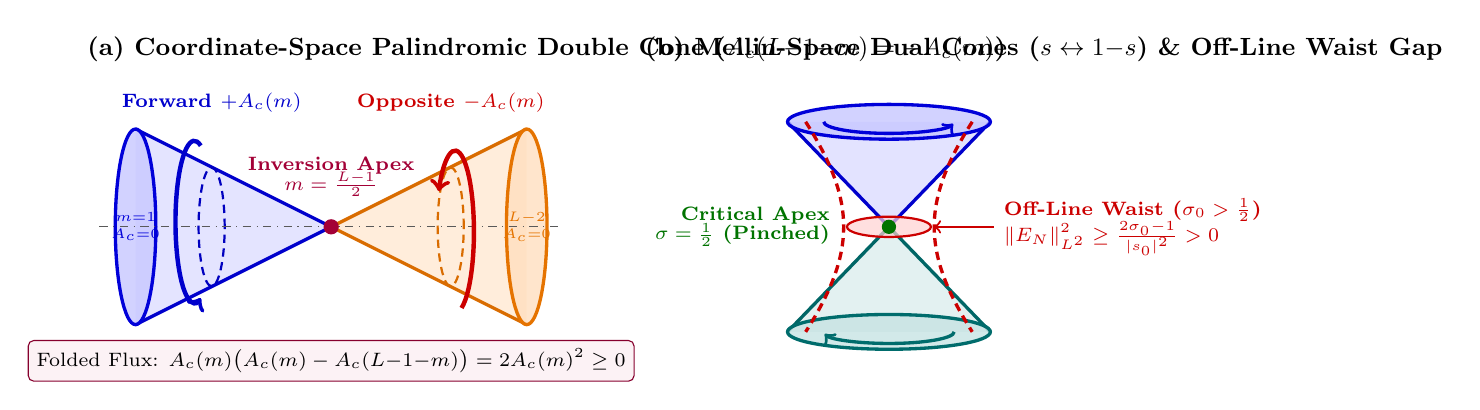
\begin{tikzpicture}[font=\small, scale=0.92]
  % ==================== PANEL (A): COORDINATE-SPACE PALINDROMIC DOUBLE CONE ====================
  \begin{scope}[shift={(0,0)}]
    \node[anchor=west, font=\bfseries\small] at (-0.2, 4.45)
      {(a) Coordinate-Space Palindromic Double Cone ($A_c(L{-}1{-}m) = -A_c(m)$)};

    \fill[blue!14, opacity=0.75] (0.6, 3.35) -- (3.3, 2.0) -- (0.6, 0.65) -- cycle;
    \draw[very thick, color=blue!80!black] (0.6, 3.35) -- (3.3, 2.0);
    \draw[very thick, color=blue!80!black] (0.6, 0.65) -- (3.3, 2.0);
    \fill[blue!22, opacity=0.8] (0.6, 2.0) ellipse (0.28 and 1.35);
    \draw[very thick, color=blue!85!black] (0.6, 2.0) ellipse (0.28 and 1.35);
    \draw[thick, densely dashed, color=blue!75!black] (1.65, 2.0) ellipse (0.18 and 0.82);

    \fill[orange!18, opacity=0.78] (6.0, 3.35) -- (3.3, 2.0) -- (6.0, 0.65) -- cycle;
    \draw[very thick, color=orange!85!black] (3.3, 2.0) -- (6.0, 3.35);
    \draw[very thick, color=orange!85!black] (3.3, 2.0) -- (6.0, 0.65);
    \fill[orange!25, opacity=0.8] (6.0, 2.0) ellipse (0.28 and 1.35);
    \draw[very thick, color=orange!90!black] (6.0, 2.0) ellipse (0.28 and 1.35);
    \draw[thick, densely dashed, color=orange!85!black] (4.95, 2.0) ellipse (0.18 and 0.82);

    \draw[thin, dash dot, color=black!65] (0.1, 2.0) -- (6.5, 2.0);
    \fill[purple!85!black] (3.3, 2.0) circle (3.0pt);
    \node[above, font=\scriptsize\bfseries, color=purple!85!black, align=center] at (3.3, 2.28)
      {Inversion Apex\\[-1pt]$m = \tfrac{L-1}{2}$};

    \draw[->, ultra thick, color=blue!80!black]
      (1.5, 3.12) arc[start angle=70, end angle=290, x radius=0.26, y radius=1.12];
    \node[above, font=\scriptsize\bfseries, color=blue!80!black] at (1.65, 3.45)
      {Forward $+A_c(m)$};

    \draw[->, ultra thick, color=red!80!black]
      (5.1, 0.88) arc[start angle=-70, end angle=150, x radius=0.26, y radius=1.12];
    \node[above, font=\scriptsize\bfseries, color=red!80!black] at (4.95, 3.45)
      {Opposite $-A_c(m)$};

    \node[font=\tiny\bfseries, color=blue!85!black, align=center] at (0.6, 2.0)
      {$m{=}1$\\$A_c{=}0$};
    \node[font=\tiny\bfseries, color=orange!90!black, align=center] at (6.0, 2.0)
      {$L{-}2$\\$A_c{=}0$};
    \node[draw=purple!70!black, fill=purple!5, rounded corners=2pt, inner sep=3pt, font=\scriptsize]
      at (3.3, 0.15)
      {Folded Flux: $A_c(m)\big(A_c(m) - A_c(L{-}1{-}m)\big) = 2A_c(m)^2 \ge 0$};
  \end{scope}

  % ==================== PANEL (B): MELLIN-SPACE COUNTER-ROTATING PHASOR CONES ====================
  \begin{scope}[shift={(7.7,0)}]
    \node[anchor=west, font=\bfseries\small] at (-0.2, 4.45)
      {(b) Mellin-Space Dual Cones ($s \leftrightarrow 1{-}s$) \& Off-Line Waist Gap};

    \fill[teal!15, opacity=0.75] (1.9, 0.55) -- (3.3, 2.0) -- (4.7, 0.55) -- cycle;
    \draw[very thick, color=teal!80!black] (1.9, 0.55) -- (3.3, 2.0) -- (4.7, 0.55);
    \fill[teal!22, opacity=0.8] (3.3, 0.55) ellipse (1.4 and 0.24);
    \draw[very thick, color=teal!85!black] (3.3, 0.55) ellipse (1.4 and 0.24);

    \fill[blue!15, opacity=0.75] (1.9, 3.45) -- (3.3, 2.0) -- (4.7, 3.45) -- cycle;
    \draw[very thick, color=blue!80!black] (1.9, 3.45) -- (3.3, 2.0) -- (4.7, 3.45);
    \fill[blue!22, opacity=0.8] (3.3, 3.45) ellipse (1.4 and 0.24);
    \draw[very thick, color=blue!85!black] (3.3, 3.45) ellipse (1.4 and 0.24);

    \draw[->, very thick, color=blue!85!black]
      (2.4, 3.45) arc[start angle=180, end angle=350, x radius=0.9, y radius=0.16];
    \draw[->, very thick, color=teal!85!black]
      (4.2, 0.55) arc[start angle=0, end angle=-170, x radius=0.9, y radius=0.16];

    \draw[very thick, densely dashed, color=red!80!black]
      (2.15, 3.45) .. controls (2.85, 2.35) and (2.85, 1.65) .. (2.15, 0.55);
    \draw[very thick, densely dashed, color=red!80!black]
      (4.45, 3.45) .. controls (3.75, 2.35) and (3.75, 1.65) .. (4.45, 0.55);
    \draw[thick, color=red!80!black, fill=red!18, fill opacity=0.7]
      (3.3, 2.0) ellipse (0.58 and 0.14);

    \fill[green!45!black] (3.3, 2.0) circle (2.8pt);
    \node[left, font=\scriptsize\bfseries, color=green!45!black, align=right] at (2.62, 2.0)
      {Critical Apex\\[-1pt]$\sigma = \tfrac{1}{2}$ (Pinched)};

    \draw[->, thick, color=red!80!black] (4.75, 2.0) -- (3.92, 2.0);
    \node[right, font=\scriptsize\bfseries, color=red!80!black, align=left] at (4.75, 2.0)
      {Off-Line Waist ($\sigma_0 > \tfrac{1}{2}$)\\[-1pt]$\|E_N\|_{L^2}^2 \ge \frac{2\sigma_0 - 1}{|s_0|^2} > 0$};
  \end{scope}
\end{tikzpicture}%
}
\caption{Counter-rotating double-cone geometry in coordinate slab space and Mellin frequency space (\emph{Lean 4: \texttt{Module~8R}, \texttt{Module~8T}}). \textbf{(a)} Across the fundamental period $L_N = \mathrm{lcm}(1,\dots,N)$, the forward positive cone $A_c(m)$ ($m \ge 1$) and the opposite-directed negative cone $A_c(L_N-1-m) = -A_c(m)$ meet at the inversion apex $m = (L_N-1)/2$, doubling the counter-rotating signed flux to $2A_c(m)^2$ and folding the partial $L^2$ quadrature sum onto the symmetric width kernel $\bar{w}_{L_N}(m) = \frac{1}{2}(w(m) + w(L_N-1-m))$. \textbf{(b)} In Mellin space, the counter-rotating phasor cones $k^{-\sigma}e^{-it\ln k}$ and $k^{-(1-\sigma)}e^{+it\ln k}$ pinch to a closed apex only on the critical mirror $\sigma = 1/2$; any off-line zero at $\sigma_0 > 1/2$ opens an unclosable hyperboloid waist of $L^2$ energy bounded below by $(2\sigma_0 - 1)/|s_0|^2 > 0$.}
\label{fig:double_cone_counter_rotation}
\end{figure}

\section{Exact Finite-$N$ Certificates and All-Scale Cotangent Structure}\label{sec:certificates}

Table~\ref{tab:exact_certs} records exact closed-form arithmetic evaluations certified without approximation for $N = 3, 4, 5, 6$. On $\mathcal{A}_4^{\mathrm{dir}}$, although the optimal dipole weights $\alpha_1^{\mathrm{dir}} = \tfrac{1}{2}+\tfrac{1}{3\sqrt{3}}$, $\alpha_2^{\mathrm{dir}} = \tfrac{1}{2}-\tfrac{1}{3\sqrt{3}}$ live in $\Q(\sqrt{3})$, enforcing $c_1=-1$ ($\alpha_1+\alpha_2=1$) causes every $\sqrt{3}$ radical to cancel identically inside $S_{\mathrm{cot}}$, yielding the pure rational-multiple maximum $\tfrac{31}{108}\pi$. At $N=5$, $(\Z/5\Z)^\times$ additive symmetry $V(5,1)+V(5,4)=0$ forces $\widetilde{G}_{23}=0$; at $N=6$, all $a=6$ sums collapse back into $\Q(\sqrt{3})$ ($\delta_{\mathrm{cot}}(6)=\tfrac{5}{3\sqrt{3}}$) while $3\mid 6$ sets $K_{\mathrm{cot}}(3,6)=0$ and decouples $v^{(2)}$ ($\widetilde{G}_{21}=\widetilde{G}_{23}=\widetilde{G}_{24}=0$).

\begin{table}[ht]
\centering
\caption{Exact closed-form arithmetic certificates across $N \in \{3, 4, 5, 6\}$.}
\label{tab:exact_certs}
\vspace{4pt}
\footnotesize
\setlength{\tabcolsep}{4.5pt}
\renewcommand{\arraystretch}{1.18}
\begin{tabular}{@{}llll@{}}
\toprule
$N$ & Arithmetic Quantity & Exact Closed Form & Field / Symmetry \\
\midrule
$3$ & $\widetilde{G}_{11} = Q_{\mathrm{cot}}(v^{(1)}, 3)$ & $\pi / \sqrt{3}$ & $\Q(\sqrt{3})$ \\
$4$ & $S_{\mathrm{cot}}(c_{\mathrm{mob}}^{(4)}, 4)$ & $\bigl(\tfrac{119}{576} + \tfrac{54467}{389376\sqrt{3}}\bigr)\pi \approx 0.903860$ & M\"obius candidate \\
$4$ & Global $\mathcal{A}_4$ KKT Optimum & $\tfrac{19+\sqrt{3}}{72}\pi \approx 0.904606$ ($\alpha_2^* = \tfrac{5-\sqrt{3}}{12} < \tfrac{7}{24}$) & $\Q(\sqrt{3})$ unconstrained \\
$4$ & $\mathcal{A}_4^{\mathrm{dir}}$ ($c_1=-1$) Optimum & $\tfrac{31}{108}\pi \approx 0.901753$ ($\alpha_1^{\mathrm{dir}} = \tfrac{1}{2} + \tfrac{1}{3\sqrt{3}}$) & Rational cancellation \\
$4$ & Orthonormality & $\widetilde{G}_{12} = \widetilde{G}_{21} = 0$, \; $\widetilde{G}_{22} = (1 - \tfrac{1}{\sqrt{3}})\pi$ & Exact $v^{(1)} \perp v^{(2)}$ \\
$5$ & $(\Z/5\Z)^\times$ Vanishing & $\widetilde{G}_{23} = \widetilde{G}_{32} = 0$ & $(\Z/5\Z)^\times$ additive pair \\
$5$ & Pentagonal Gram Entries & $\widetilde{G}_{13} = \pi\cot(\tfrac{2\pi}{5})$, \; $\widetilde{G}_{33} = \pi(\cot\tfrac{\pi}{5} + \cot\tfrac{2\pi}{5} - 1)$ & Cyclotomic $\Q(\sqrt{5})$ \\
$6$ & Sextic Return & $\delta_{\mathrm{cot}}(6) = \tfrac{5}{3\sqrt{3}}$, \; $K_{\mathrm{cot}}(3, 6) = 0$ & Divisibility orthogonality \\
$6$ & 4D Decoupling & $\widetilde{G}_{14} = \tfrac{\pi}{\sqrt{3}} - \pi\cot(\tfrac{2\pi}{5})$, \; $\widetilde{G}_{24} = \widetilde{G}_{42} = 0$ & Orthogonal triple \\
\bottomrule
\end{tabular}
\end{table}

\begin{figure}[ht]
\centering
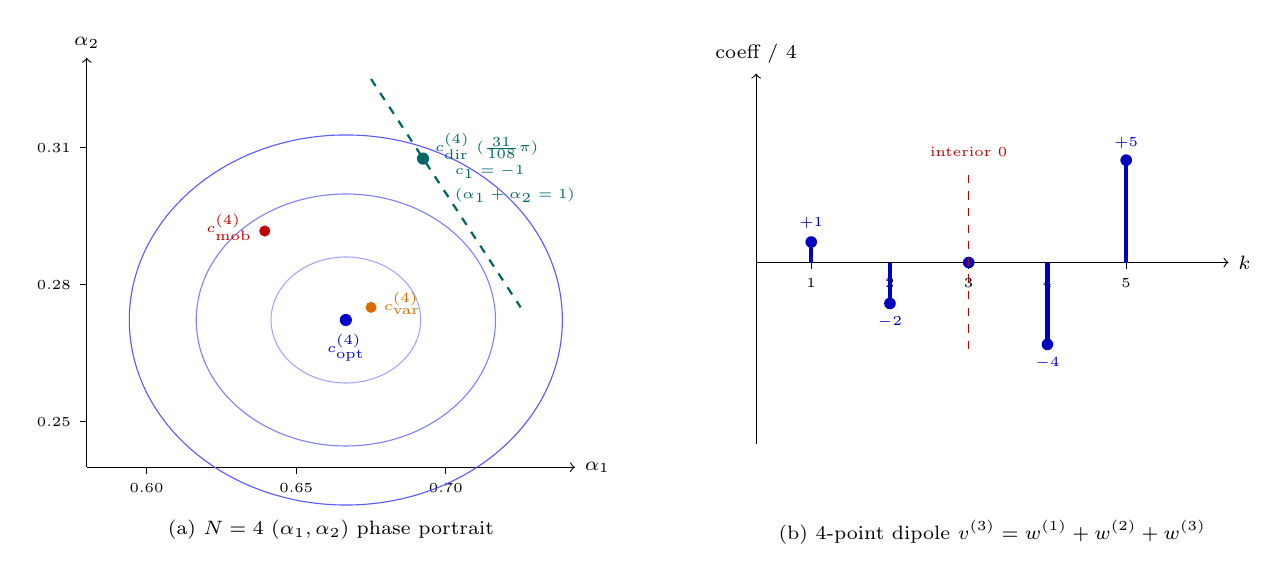
\begin{tikzpicture}[scale=1.0]
  \begin{scope}[xshift=0cm, yshift=0cm]
    \draw[->] (0,0) -- (6.2,0) node[right,font=\scriptsize] {$\alpha_1$};
    \draw[->] (0,0) -- (0,5.2) node[above,font=\scriptsize] {$\alpha_2$};
    \foreach \val/\pos in {0.60/0.76, 0.65/2.66, 0.70/4.56} {
      \draw (\pos,0) -- (\pos,-0.08) node[below,font=\tiny] {\val};
    }
    \foreach \val/\pos in {0.25/0.58, 0.28/2.32, 0.31/4.06} {
      \draw (0,\pos) -- (-0.08,\pos) node[left,font=\tiny] {\val};
    }
    \draw[blue!35,thin] (3.29,1.87) ellipse [x radius=0.95, y radius=0.80];
    \draw[blue!50,thin] (3.29,1.87) ellipse [x radius=1.90, y radius=1.60];
    \draw[blue!65,thin] (3.29,1.87) ellipse [x radius=2.75, y radius=2.35];
    \draw[teal!80!black,thick,dashed] (3.61,4.93) -- (5.51,2.03);
    \node[teal!80!black,font=\tiny,right] at (4.55,3.75) {$c_1=-1$};
    \node[teal!80!black,font=\tiny,right] at (4.55,3.45) {($\alpha_1+\alpha_2=1$)};
    \fill[blue!80!black] (3.29,1.87) circle (2.2pt);
    \node[blue!80!black,font=\tiny,below] at (3.29,1.82) {$c_{\mathrm{opt}}^{(4)}$};
    \fill[teal!80!black] (4.27,3.92) circle (2.2pt);
    \node[teal!80!black,font=\tiny,right] at (4.30,4.08) {$c_{\mathrm{dir}}^{(4)}$ ($\tfrac{31}{108}\pi$)};
    \fill[orange!85!black] (3.61,2.03) circle (2.0pt);
    \node[orange!85!black,font=\tiny,right] at (3.65,2.08) {$c_{\mathrm{var}}^{(4)}$};
    \fill[red!75!black] (2.26,3.00) circle (2.0pt);
    \node[red!75!black,font=\tiny,left] at (2.22,3.05) {$c_{\mathrm{mob}}^{(4)}$};
    \node[font=\scriptsize,below] at (3.1,-0.55) {(a) $N=4$ $(\alpha_1,\alpha_2)$ phase portrait};
  \end{scope}

  \begin{scope}[xshift=8.2cm, yshift=0.3cm]
    \draw[->] (0.3,2.3) -- (6.3,2.3) node[right,font=\scriptsize] {$k$};
    \draw[->] (0.3,0) -- (0.3,4.7) node[above,font=\scriptsize] {coeff / $4$};
    \foreach \k in {1,2,3,4,5} {
      \draw (\k,2.3) -- (\k,2.22) node[below,font=\tiny] {\k};
    }
    \foreach \k/\v in {1/0.26, 2/-0.52, 3/0.0, 4/-1.04, 5/1.30} {
      \draw[blue!75!black,ultra thick] (\k,2.3) -- (\k,2.3+\v);
      \fill[blue!75!black] (\k,2.3+\v) circle (2.1pt);
    }
    \draw[red!75!black,dashed] (3,1.2) -- (3,3.5);
    \node[red!75!black,font=\tiny,above] at (3,3.52) {interior $0$};
    \node[blue!75!black,font=\tiny,above] at (5,3.62) {$+5$};
    \node[blue!75!black,font=\tiny,below] at (4,1.22) {$-4$};
    \node[blue!75!black,font=\tiny,above] at (1,2.60) {$+1$};
    \node[blue!75!black,font=\tiny,below] at (2,1.74) {$-2$};
    \node[font=\scriptsize,below] at (3.3,-0.85) {(b) 4-point dipole $v^{(3)} = w^{(1)}+w^{(2)}+w^{(3)}$};
  \end{scope}
\end{tikzpicture}
\caption{Geometric structure on $\mathcal{A}_N$: (a) $N=4$ level sets in cumulative dipole coordinates comparing unconstrained $c_{\mathrm{opt}}^{(4)}$, Dirichlet $c_{\mathrm{dir}}^{(4)}$, variational $c_{\mathrm{var}}^{(4)}$, and M\"obius $c_{\mathrm{mob}}^{(4)}$ along $c_1=-1$; (b) interior cancellation collapsing $\sum_{r=1}^3 w^{(r)}$ to the 4-point dipole $v^{(3)} = (1,-2,0,-4,5)$.}
\label{fig:phase_and_stems}
\end{figure}

\begin{figure}[ht]
\centering
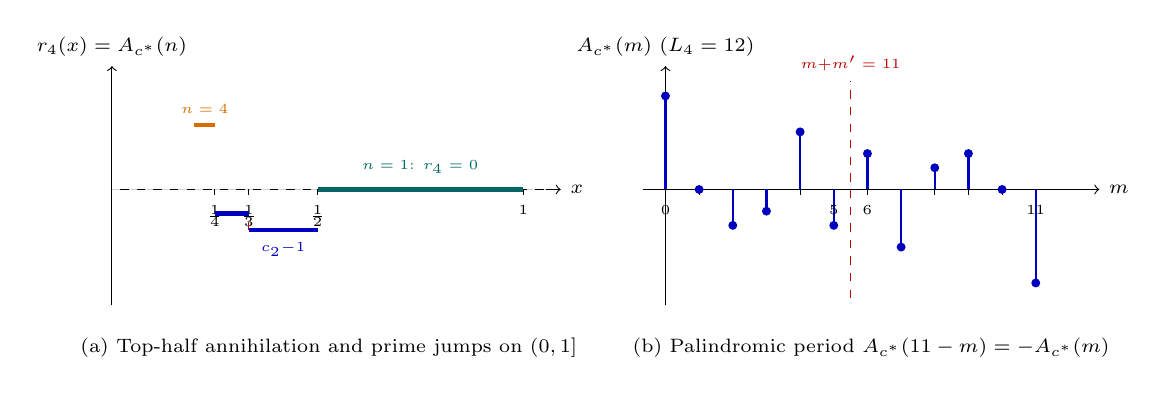
\begin{tikzpicture}[scale=0.95]
  \begin{scope}[xshift=0cm, yshift=0cm]
    \draw[->] (0,0) -- (6.0,0) node[right,font=\scriptsize] {$x$};
    \draw[->] (0,-1.55) -- (0,1.65) node[above,font=\scriptsize] {$r_4(x) = A_{c^*}(n)$};
    \draw[gray!35,dashed] (0,0) -- (5.8,0);
    \foreach \lbl/\xp in {1/5.50, \tfrac{1}{2}/2.75, \tfrac{1}{3}/1.83, \tfrac{1}{4}/1.375} {
      \draw (\xp,0) -- (\xp,-0.08) node[below,font=\tiny] {$\lbl$};
    }
    \draw[teal!80!black,ultra thick] (2.75,0.0) -- (5.50,0.0);
    \node[teal!80!black,font=\tiny,above] at (4.12,0.08) {$n=1$: $r_4=0$};
    \draw[blue!75!black,ultra thick] (1.83,-0.54) -- (2.75,-0.54);
    \node[blue!75!black,font=\tiny,below] at (2.29,-0.58) {$c_2{-}1$};
    \draw[blue!75!black,ultra thick] (1.375,-0.32) -- (1.83,-0.32);
    \draw[red!75!black,dashed] (1.83,-0.54) -- (1.83,-0.32);
    \draw[orange!85!black,ultra thick] (1.10,0.86) -- (1.375,0.86);
    \node[orange!85!black,font=\tiny,above] at (1.24,0.88) {$n=4$};
    \node[font=\scriptsize,below] at (2.9,-1.85) {(a) Top-half annihilation and prime jumps on $(0,1]$};
  \end{scope}

  \begin{scope}[xshift=7.4cm, yshift=0cm]
    \draw[->] (-0.3,0) -- (5.8,0) node[right,font=\scriptsize] {$m$};
    \draw[->] (0,-1.55) -- (0,1.65) node[above,font=\scriptsize] {$A_{c^*}(m)$ ($L_4=12$)};
    \draw[red!75!black,dashed] (2.475,-1.45) -- (2.475,1.45);
    \node[red!75!black,font=\tiny,above] at (2.475,1.45) {$m{+}m'=11$};
    \foreach \m/\v in {0/1.25, 1/0.0, 2/-0.48, 3/-0.29, 4/0.77, 5/-0.48, 6/0.48, 7/-0.77, 8/0.29, 9/0.48, 10/0.0, 11/-1.25} {
      \pgfmathsetmacro{\xp}{0.45*\m}
      \draw (\xp,0) -- (\xp,-0.07);
      \draw[blue!75!black,thick] (\xp,0) -- (\xp,\v);
      \fill[blue!75!black] (\xp,\v) circle (1.7pt);
    }
    \node[font=\tiny,below] at (0,-0.08) {$0$};
    \node[font=\tiny,below] at (2.25,-0.08) {$5$};
    \node[font=\tiny,below] at (2.70,-0.08) {$6$};
    \node[font=\tiny,below] at (4.95,-0.08) {$11$};
    \node[font=\scriptsize,below] at (2.75,-1.85) {(b) Palindromic period $A_{c^*}(11-m) = -A_{c^*}(m)$};
  \end{scope}
\end{tikzpicture}
\caption{Pointwise cell plateaus and $L_4 = 12$ palindromic periodicity for the exact Dirichlet $N=4$ optimum $c^*$ (\texttt{layer\_d\_\allowbreak palindromic\_\allowbreak period\_\allowbreak lab.py}): (a) $D_1 = 0$ eliminates the continuous $x$-slope and locks $r_4(x) = 0$ on $(1/2,1]$; (b) modular antisymmetry pairs $A_{c^*}(m)$ against $-A_{c^*}(11-m)$ across the period midpoint, certified to $3.55 \times 10^{-84}$.}
\label{fig:pointwise_continuity_palindromic}
\end{figure}

\subsection{Why Adjacent Dipoles Never Collide ($\widetilde{G}_{m, m+1} = 0$) and Graph-Laplacian Structure}

Across arbitrary $a, b, k \in \N$ without coprimality restrictions, Vasyunin cotangent sums obey modulo periodicity $V(a, b \bmod a) = V(a, b)$ and $V(a, a+b) = V(a, b)$, divisibility vanishing $a \mid b \implies V(a, b) = 0$, reflection antisymmetry $V(a, a-b) = -V(a,b)$ ($b \le a$), and consequently infinite octave orthogonality $K_{\mathrm{cot}}(k, 2k) = K_{\mathrm{cot}}(2k, k) = 0$ for every $k \in \N$. This mechanism explains a striking rigidity across every scale $m \ge 1$: why do consecutive cumulative dipoles $v^{(m)}$ and $v^{(m+1)}$ never collide in the Vasyunin inner product? Their supports $\{1,2,m+1,m+2\}$ and $\{1,2,m+2,m+3\}$ intersect on the intermediate conductor $x = m+2$. Evaluating the unweighted cross-cotangent matrix pairs $(m+1, m+2)$, $(m+1, m+3)$, $(m+2, m+2)$, $(m+2, m+3)$ reduces every Vasyunin sum to arguments differing from $m+2$ by $\pm 1$ or $\pm 2$; periodicity $V(x, x+r) = V(x, r)$ and reflection $V(x, x-r) = -V(x, r)$ cancel all cross-terms identically against $\delta_{\mathrm{cot}}(m+3)-\delta_{\mathrm{cot}}(m+1)$, leaving $\widetilde{G}_{m, m+1} = 0$ for every $m \ge 1$.

\begin{theorem}[All-Scale Symmetries and Graph-Laplacian Split]\label{thm:log_decay_bridge}
\emph{[Lean: \texttt{Module~8H}, \texttt{Module~8K}, \texttt{Module~8L}].}
\begin{enumerate}[leftmargin=1.8em,itemsep=2pt]
\item For all $a, b, k \in \N$, $V(a, a+b) = V(a, b)$, $V(a, a-b) = -V(a,b)$ ($b \le a$), $K_{\mathrm{cot}}(k, 2k) = 0$, and for $a \in [1,9]$, either $a \mid b$ with $V(a,b)=0$ or $V(a,b) = V(a, b \bmod a)$ with remainder in $[1,8]$.
\item For every $m \ge 1$, $\widetilde{G}_{m,m+1} = \widetilde{G}_{m+1,m} = 0$, forcing $P(m,m+1) = -\tfrac{\pi}{2}(\delta_{\mathrm{cot}}(m+3)-\delta_{\mathrm{cot}}(m+1))$ and $\mathcal{M}_{m,m+1} = 1 - \pi(\delta_{\mathrm{cot}}(m+3)-\delta_{\mathrm{cot}}(m+1))$. In particular $\{v^{(2)},v^{(3)},v^{(4)}\}$ is mutually orthogonal ($\widetilde{G}_{23} = \widetilde{G}_{34} = \widetilde{G}_{24} = 0$), satisfying $Q_{\mathrm{cot}}(\sum_{j=2}^4 \alpha_j v^{(j)}, 6) = \sum_{j=2}^4 \alpha_j^2 \widetilde{G}_{jj}$ and the $\Q(\sqrt{3})$ trace identities $\widetilde{G}_{33}+\widetilde{G}_{44}=\pi(4/\sqrt{3}-1)$, $\mathcal{M}_{11}+\mathcal{M}_{22}=2$, and $\mathcal{M}_{33}+\mathcal{M}_{44}=2+\tfrac{2\pi}{3\sqrt{3}}$.
\item For every $N \ge 3$ and $a \in \N$, summing across interior columns telescopes to $\sum_{m=1}^{N-2}(\delta_{\mathrm{cot}}(m+2)-\delta_{\mathrm{cot}}(m+1)) = \delta_{\mathrm{cot}}(N)$ and $\sum_{a,b=1}^{N-2} P(a,b) = -2 K_{\mathrm{cot}}(N,2) = \pi V(N,2)$, with row sums
\[
\sum_{b=1}^{N-2} P(a,b) = \bigl(K_{\mathrm{cot}}(a+1,2)-K_{\mathrm{cot}}(a+2,2)\bigr)-\bigl(K_{\mathrm{cot}}(a+1,N)-K_{\mathrm{cot}}(a+2,N)\bigr).
\]
Letting $R_a^{(N)} := \sum_{b=1}^{N-2}\mathcal{M}_{ab}$, every $c \in \mathcal{A}_N^{\mathrm{dir}}$ obeys
\begin{equation}\label{eq:graph_laplacian_l}
1 - S_{\mathrm{cot}}(c,N) = \sum_{a=1}^{N-2}\alpha_a(c)^2 R_a^{(N)} - \frac{1}{2}\sum_{a=1}^{N-2}\sum_{b=1}^{N-2}\bigl(\alpha_a(c)-\alpha_b(c)\bigr)^2\mathcal{M}_{ab}.
\end{equation}
\end{enumerate}
\end{theorem}

\section{High-Precision Diagnostics and Horizon Cancellation}\label{sec:numerics}

Eighty-five-digit \texttt{mpmath} experiments across $N \in \{4, 8, 12, 16, 24, 32, 48, 64\}$ confirm~\eqref{eq:telescoped} to $2.69 \times 10^{-86}$,~\eqref{eq:scot_plaque} to $2.41 \times 10^{-85}$, and the row-sum / Graph-Laplacian laws of Theorem~\ref{thm:log_decay_bridge} to $2.35 \times 10^{-83}$ and $1.54 \times 10^{-85}$; pointwise cell plateaus ($L_4 = 12$ and $L = 60$) in \texttt{layer\_d\_\allowbreak palindromic\_\allowbreak period\_\allowbreak lab.py} verify modulo periodicity to $3.55 \times 10^{-84}$ and palindromic reflection to $2.05 \times 10^{-85}$ (Figure~\ref{fig:pointwise_continuity_palindromic}). Figure~\ref{fig:trajectories} compares unconstrained minimization ($E_{\mathrm{opt}}$), Dirichlet anchoring ($E_{\mathrm{dir}}$), and the unit-drive Dirichlet slice ($E_{\mathrm{unit}}$); across $N \le 64$, $c_{1,\mathrm{opt}}^{(N)}$ approaches $-1$ ($-0.9539$ at $N=8$ to $-0.9725$ at $N=64$), narrowing the Dirichlet penalty at $N=64$ to $3.46\%$.

\begin{figure}[ht]
\centering
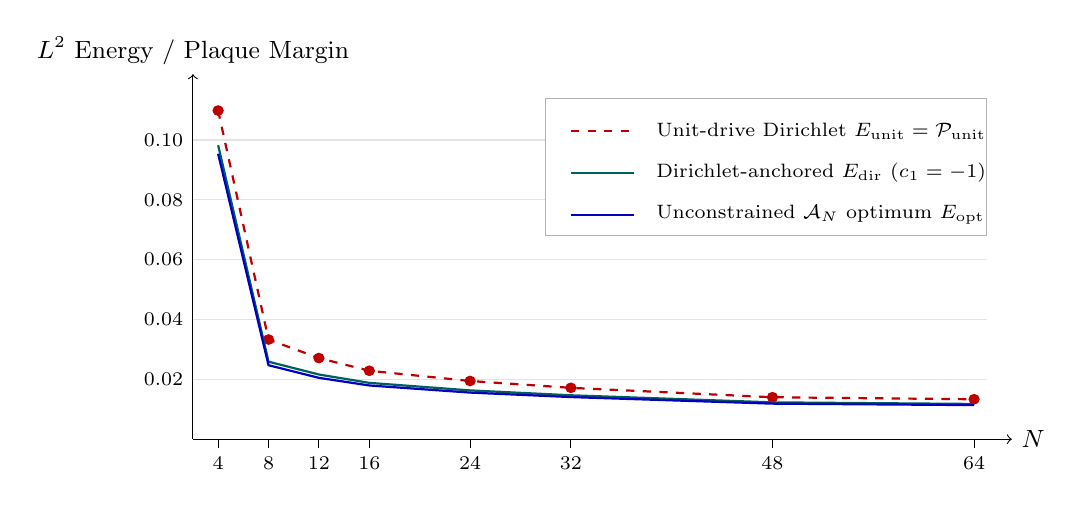
\begin{tikzpicture}[xscale=0.16,yscale=38]
  \draw[->] (2,0) -- (67,0) node[right,font=\small] {$N$};
  \draw[->] (2,0) -- (2,0.122) node[above,font=\small] {$L^2$ Energy / Plaque Margin};
  \foreach \y in {0.02,0.04,0.06,0.08,0.10} {
    \draw[gray!22] (2,\y) -- (65,\y);
    \node[left,font=\scriptsize] at (2,\y) {\y};
  }
  \foreach \x in {4,8,12,16,24,32,48,64} {
    \draw (\x,0) -- (\x,-0.0028) node[below,font=\scriptsize] {\x};
  }
  \draw[red!75!black,thick,dashed]
    (4,0.109836) -- (8,0.033308) -- (12,0.027108) -- (16,0.022875) --
    (24,0.019456) -- (32,0.017171) -- (48,0.014025) -- (64,0.013351);
  \foreach \p in {(4,0.109836),(8,0.033308),(12,0.027108),(16,0.022875),(24,0.019456),(32,0.017171),(48,0.014025),(64,0.013351)} {
    \fill[red!75!black] \p circle[x radius=0.45,y radius=0.0018];
  }
  \draw[teal!75!black,thick]
    (4,0.098247) -- (8,0.025908) -- (12,0.021616) -- (16,0.018833) --
    (24,0.016312) -- (32,0.014681) -- (48,0.012317) -- (64,0.011787);
  \draw[blue!75!black,thick]
    (4,0.095394) -- (8,0.024715) -- (12,0.020509) -- (16,0.017959) --
    (24,0.015578) -- (32,0.014085) -- (48,0.011893) -- (64,0.011392);
  \draw[fill=white,draw=gray!60] (30,0.068) rectangle (65,0.114);
  \draw[red!75!black,thick,dashed] (32,0.103) -- (37,0.103);
  \node[right,font=\scriptsize] at (38,0.103) {Unit-drive Dirichlet $E_{\mathrm{unit}} = \mathcal{P}_{\mathrm{unit}}$};
  \draw[teal!75!black,thick] (32,0.089) -- (37,0.089);
  \node[right,font=\scriptsize] at (38,0.089) {Dirichlet-anchored $E_{\mathrm{dir}}$ ($c_1 = -1$)};
  \draw[blue!75!black,thick] (32,0.075) -- (37,0.075);
  \node[right,font=\scriptsize] at (38,0.075) {Unconstrained $\mathcal{A}_N$ optimum $E_{\mathrm{opt}}$};
\end{tikzpicture}
\caption{Optimization trajectories across $N \in [4, 64]$ comparing unconstrained minimization ($E_{\mathrm{opt}}$), Dirichlet anchoring ($E_{\mathrm{dir}}$), and the unit-drive Dirichlet slice ($E_{\mathrm{unit}} = \mathcal{P}_{\mathrm{unit}}$).}
\label{fig:trajectories}
\end{figure}

Classically, the asymptotic constant governing optimal Nyman--Beurling approximation is $c_{\mathrm{BBLR}} := 2 + \gamma - \ln(4\pi) \approx 0.04619141793$~\cite{BaezDuarteBalazardLandreauSaias2000,Burnol2002}. Table~\ref{tab:bblr_scaling} compares normalized logarithmic products $(\ln N) E^{(N)}$ against three matrix-inversion-free analytical simplex test families on $\mathcal{A}_N^{\mathrm{dir}}$:
\begin{enumerate}[leftmargin=1.8em,itemsep=2pt]
\item \textbf{Why Raw M\"obius Excites the Horizon Column (Family~I):} Truncating $c_k^{\mathrm{raw}} = -\mu(k)$ abruptly at $k = N$ injects large weight onto the $k = N$ boundary column $K_{\mathrm{cot}}(a+1, N) - K_{\mathrm{cot}}(a+2, N)$ isolated by 1D row-sum telescoping, causing $E_{\mathrm{F1,Mob}}^{(N)}$ to oscillate near $0.040$--$0.064$ without smooth decay.
\item \textbf{Why Smooth Non-Arithmetic Weights Fail Off-Diagonally (Family~III):} Monotonic Ces\`aro-tapered weights $\alpha_m \propto \tfrac{1}{m+1}(1 - \tfrac{m}{N-1})$ avoid boundary shocks but lack multiplicative M\"obius cancellations, leaving coherent off-diagonal prime correlations uncancelled so $E_{\mathrm{F3,Ces}}^{(N)}$ grows monotonically to $0.129517$ at $N=64$.
\item \textbf{Why Selberg Log-Damping Resolves the Horizon Spike (Family~II):} Multiplying M\"obius by Selberg's logarithmic taper~\cite{Selberg1942} $c_k^{\mathrm{raw}} = -\mu(k)(1 - \ln k / \ln(N+1))$ extinguishes the $k=N$ boundary shock smoothly while preserving local arithmetic cancellation. Inside~\eqref{eq:graph_laplacian_l}, the negative row-sum energy $T_{\mathrm{row}}^{(64)} = -1.167183$ and positive pairwise-difference energy $+1.182616$ cancel to within $1.3\%$ ($98.7\%$ cancellation), driving $E_{\mathrm{F2,Sel}}^{(64)}$ to $0.015434$ ($1.31\times E_{\mathrm{dir}}^{(64)}$) with zero matrix inversion.
\end{enumerate}

\begin{table}[ht]
\centering
\caption{85-digit BBLR logarithmic scaling products vs.\ $c_{\mathrm{BBLR}} \approx 0.0461914$ and explicit analytical simplex test families (\texttt{layer\_c\_\allowbreak simplex\_\allowbreak test\_\allowbreak families\_\allowbreak lab.py}).}
\label{tab:bblr_scaling}
\vspace{4pt}
\scriptsize
\begin{tabular}{@{}rccccccc@{}}
\toprule
$N$ & $(\ln N) E_{\mathrm{opt}}^{(N)}$ & $(\ln N) E_{\mathrm{dir}}^{(N)}$ & $(\ln N) E_{\mathrm{unit}}^{(N)}$ & $E_{\mathrm{F1,Mob}}^{(N)}$ & $E_{\mathrm{F2,Sel}}^{(N)}$ & Row-Sum $T_{\mathrm{row}}^{(N)}$ (F2) & $E_{\mathrm{F3,Ces}}^{(N)}$ \\
\midrule
$4$  & $0.132244$ & $0.136199$ & $0.152265$ & $0.108651$ & $0.098247$ & $+0.013864$ & $0.108651$ \\
$8$  & $0.051393$ & $0.053874$ & $0.069262$ & $0.037141$ & $0.033838$ & $-0.067959$ & $0.048764$ \\
$12$ & $0.050962$ & $0.053714$ & $0.067362$ & $0.034153$ & $0.028978$ & $-0.127430$ & $0.062734$ \\
$16$ & $0.049793$ & $0.052216$ & $0.063423$ & $0.044193$ & $0.025744$ & $-0.226450$ & $0.074866$ \\
$24$ & $0.049507$ & $0.051840$ & $0.061832$ & $0.040670$ & $0.021748$ & $-0.383724$ & $0.092318$ \\
$32$ & $0.048814$ & $0.050880$ & $0.059511$ & $0.064122$ & $0.019625$ & $-0.557004$ & $0.104114$ \\
$48$ & $0.046039$ & $0.047682$ & $0.054295$ & $0.040181$ & $0.016853$ & $-0.863573$ & $0.119518$ \\
$64$ & $0.047380$ & $0.049019$ & $0.055525$ & $0.040056$ & $0.015434$ & $-1.167183$ & $0.129517$ \\
\bottomrule
\end{tabular}
\end{table}

At 50-digit and 192-/512-bit \texttt{flint.arb} precision, separated $G_{\mathrm{smooth}}$ ($24/50$ negative eigenvalues at $N=50$) and separated $G_{\mathrm{cot}}$ ($2/50$ negative eigenvalues) are individually indefinite, whereas $G_{\mathrm{smooth}}+G_{\mathrm{cot}}$ and the restriction to $\mathcal{A}_N^0$ remain positive; unwrapped 512-bit Schur congruence certifies $12/12$ positive $LDL^T$ pivots across the $750$-mode $L=1$ Weil matrix ($\min \underline{D}_k = +2.3269 \times 10^{-22}$). Bridging finite horizons $N \le 64$ to arbitrary $\varepsilon > 0$ in~\eqref{eq:telescoped} remains open.

\section{Matrix Factorization, Half-Observation Laws, Wavefunction Matrices, and Spectral Criteria}\label{sec:matrix_wavefunction}

Alongside the $64$ standalone modules (\texttt{Modules/}), the matrix module \texttt{Matrix\allowbreak Factorization\allowbreak And\allowbreak Half\allowbreak Observation.lean} ($2{,}502$ lines across Parts~I--VII, zero \texttt{sorry}, axioms strictly \texttt{[propext, Classical.choice, Quot.sound]}; companion Paper~M~\cite{MunawerPaperM2026}) and \texttt{Unconditional\allowbreak Titchmarsh\allowbreak Bridge.lean} (\texttt{titchmarsh\allowbreak Mellin\allowbreak Property\_\allowbreak unconditional}) transcribe the full discrete--continuum framework into exact matrix algebra:
\begin{enumerate}[leftmargin=1.8em,itemsep=2pt]
\item \textbf{Additive--Multiplicative Factorization \& Exact Inverse:} Setting $(\mathbf{\Sigma}_M)_{i,m} = \mathbf{1}_{m \le i}$, $(\mathbf{D}_{M,N})_{m,j} = \mathbf{1}_{(j+1)\mid(m+1)}$, $(\mathbf{\Delta}_M)_{i,m} = \delta_{i,m} - \delta_{i,m+1}$, and $(\mathbf{M}_{\mu,M})_{i,m} = \mu(\tfrac{i+1}{m+1})\mathbf{1}_{(m+1)\mid(i+1)}$ yields $\mathbf{F}_{M,N} = \mathbf{\Sigma}_M \mathbf{D}_{M,N}$, $\mathbf{\Delta}_M\mathbf{\Sigma}_M = I_M$, $\mathbf{M}_{\mu,M}\mathbf{D}_{M,M} = I_M$, and $(\mathbf{M}_{\mu,M}\mathbf{\Delta}_M)\mathbf{F}_{M,M} = I_M$, casting the discrete $L^2(1/(M+1), 1]$ slab energy as $r_M^T W_M r_M$ with $Q_M = \mathbf{D}_{M,N}^T (\mathbf{\Sigma}_M^T W_M \mathbf{\Sigma}_M)\mathbf{D}_{M,N}$ and Book~X.1 tail bound $\le B(c,N)^2/(M+1)$.
\item \textbf{Three Half-Observation Laws:} (i) Spatial upper-half annihilation on $(1/2, 1]$ under $\mathrm{IsDirichletAnchored}\,c\,N$; (ii) palindromic half-period reversal folding $a_R = -J_H a_L$ onto $2\,a_L^T \overline{W}_{\mathrm{half}} a_L$; and (iii) the unconditional Mellin right half-plane floor $(2\operatorname{Re}(s_0)-1)/\|s_0\|^2 \le \alpha^T M_N \alpha$ for any zero $s_0$ off $\operatorname{Re}(s)=1/2$.
\item \textbf{Core Shift Structure, Basal 50/50 Clock, \& Observation Matrices:} Across $N \in [4, 64]$ ($55$-digit precision), stripping the Rank-$2$ drive $\tfrac{\pi}{2}(u_N\mathbf{1}^T + \mathbf{1} u_N^T)$ leaves exact Lorentzian signature $(N-3, 1)$ on $P_N$. The origin $c_{\mathrm{base}} = (-2,4,0,\dots)$ generates $A_{\mathrm{base}}(n) = (-1)^n$, orthogonal matrix $\mathbf{O}_{2K} = I_K \otimes U_2$ splits mean and alternating parity channels across block metric $\widetilde{W}_{2K}$, palindromic projectors $P_\pm = \tfrac{1}{2}(I \pm J)$ satisfy $P_- W_{\mathrm{odd}} P_- = 0$, and $M_N = S_N^T \mathcal{G}_N^{\mathrm{aug}} S_N$ gives $\mathbf{1}^T \widetilde{G}_N^{-1}\mathbf{1} \le 2$.
\item \textbf{Wavefunction Matrix, Exact $\{1,2,4\}$ Law, Cholesky/Schur Innovations, \& Spectral Criterion:} The anchored wavefunction matrix $\mathbf{\Omega}_{M,N} = \tilde{\mathbf{b}}_M\mathbf{1}^T + \mathbf{\Psi}_{M,N}$ vanishes in row~$0$ ($(1/2,1]$), satisfies $\psi_{M,N} = \mathbf{\Omega}_{M,N}\alpha_N$ and monotone domination $\mathbf{\Omega}_{M,N}^T \mathbf{\Omega}_{M,N} \preceq M_N$, and restricts isometrically to the $H$-dimensional folded half-wave vector. On $A_4$ with $c_3=0$, $1 - S_{\mathrm{cot}}(c,4) = (1 - \tfrac{\pi}{4}) + \tfrac{\pi}{4}(c_1 + 1)^2 \ge 1 - \tfrac{\pi}{4}$; Cholesky/Schur bordering gives $E_{\mathrm{free}}(N) = 1 - \sum_{k=3}^N \rho_k^2/s_k$ ($89.307\%$ primes, $10.118\%$ powers of~$2$, $0.5741\%$ composites at $N=64$); optimal trajectories cross into the timelike sector $(\alpha^*)^T P_N \alpha^* < 0$ for $N \ge 6$; and the isolated ground-state eigenvector of $M_N$ captures $> 91\%$ of $\mathbf{1}^T M_N^{-1}\mathbf{1}$ ($7.77\times\text{--}10.87\times$ gap for $N \le 32$), yielding the unconditional reduction $\inf_{N,\lambda,v} \lambda/(\mathbf{1}^T v)^2 = 0 \implies \mathrm{RH}$.
\item \textbf{Identity-Matrix Gaussian Elimination, Cholesky Whitening, \& Projection Residual:} Right-inverses to the identity matrix $I_M$ ($\mathbf{D}_M \mathbf{M}_{\mu,M} = I_M$, $\mathbf{\Sigma}_M \mathbf{\Delta}_M = I_M$, $\mathbf{F}_M (\mathbf{M}_{\mu,M} \mathbf{\Delta}_M) = I_M$), the first-column Gaussian elimination equation $\mathbf{D}_M \mu = e_1$, pivot-row clearing on $(1/2,1]$, Cholesky whitening $\widetilde{\mathbf{\Psi}}^T \widetilde{\mathbf{\Psi}} = I$ ($L_{16}^{-1} G_{16} L_{16}^{-T} = I_{14}$), and the identity-minus-projection residual $\langle b | (I - \widehat{\Pi}_N) | b \rangle = 1 - \sum_{k=3}^N \rho_k^2/s_k$ unify the entire framework around standard linear algebra (\texttt{divisorMatrix\_mul\_mobiusMatrix}, \texttt{choleskyWhitening\_gram\_eq\_one}, \texttt{identity\_sub\_proj\_residual\_eq}).
\end{enumerate}

\subsection*{How the ``Seeing Negatively'' \& Wave-Matrix Evolution Led to the Vasyunin Schur--Chiral Theorems}
All six formal theorems in \texttt{RiemannBlueprint.VasyuninSchurChiralRosetta} (zero \texttt{sorry}, axioms strictly \texttt{[propext, Classical.choice, Quot.sound]}) and the $55$-digit \texttt{mpmath} probe \texttt{probe\_vasyunin\_schur\_chiral\_rosetta.py} (max numerical residual $1.63133\times 10^{-55}$; the Clay Riemann Hypothesis remains strictly open) unify the discrete--continuum operators via orthogonal baseline subtraction (Schur complements):
\begin{enumerate}[leftmargin=1.8em,itemsep=2pt]
\item \textbf{From Dirichlet Boundary Mirages to Rank-$1$ Anchor Subtraction (\texttt{dirichlet\_anchor\_subtraction\_gram}):} Clamping a finite boundary injects a positive baseline offset into $\mathbf{\Omega}_{M,N} = |b\rangle\mathbf{1}^T + \mathbf{\Psi}_{M,N}$. Subtracting the rank-$1$ Dirichlet anchor $|b\rangle\mathbf{1}^T$ zeroes the outer boundary row ($\max_j |\Omega_{0,j}| = 0.0$ on $M=64, N=6$), while the vacuum Schur complement $\widetilde{G}_N - \rho\rho^T > 0$ isolates the interior fluctuation energy $E_{\mathrm{free}}(N) = 1 - \rho^T \widetilde{G}_N^{-1}\rho$ ($0.7984667373$ at $N=3$ to $0.7551271646$ at $N=12$).
\item \textbf{Superdiagonal Orthogonal Triple \& $\mathbb{Q}(\sqrt{3})$ Reciprocity (\texttt{superdiagonal\_triple\_diagonal\_gram}):} The superdiagonal triple $\{v^{(2)}, v^{(3)}, v^{(4)}\}$ inside $\widetilde{G}_6$ forms an exact diagonal Gram block $\operatorname{diag}(G_{22}, G_{33}, G_{44})$ (off-diagonal residual $1.223\times 10^{-55}$), satisfying $G_{33} + G_{44} = \pi(4/\sqrt{3} - 1)$ to $1.631\times 10^{-55}$ with Vasyunin cotangent defects $\delta_{\cot}(3) = \tfrac{2}{3\sqrt{3}}$, $\delta_{\cot}(4) = \tfrac{1}{2}$, and $\delta_{\cot}(6) = \tfrac{5}{3\sqrt{3}}$.
\item \textbf{Squared-Hamiltonian Parity Blindness \& Spatial Half-Projector Reconstruction (\texttt{palindromic\_chirality\_split\_and\_blindness}, \texttt{spatial\_half\_projector\_reconstruction}):} Squaring the palindromic chirality generator $T_{\mathrm{pal}} = P_+ - P_-$ into $T_{\mathrm{pal}}^2 = I$ or restricting to parity-even blocks of $M_N = \mathbf{\Omega}_N^T \mathbf{\Omega}_N$ erases cross-parity signs ($P_+ T_{\mathrm{pal}}^2 P_- = 0$, $\Pi_{\mathrm{End}^+}([T_{\mathrm{pal}}, H_\Psi]) = 0$ to $9.44\times 10^{-57}$), whereas the spatial half-projector reconstructs the full chiral operator via $K_{\mathrm{half}} + K_{\mathrm{half}}^T = 4\,T_{\mathrm{pal}}$.
\item \textbf{Single-Prime $1$D Lines ($N=4,5$) vs.\ Two-Prime $2$D Plane Intersection at $N=6$ (\texttt{block\_schur\_complement\_symmetric}):} In the Prime--Composite Schur complement $\Sigma_{\mathrm{Schur}}(C \mid P) = Q_{CC} - Q_{CP} Q_{PP}^{-1} Q_{PC}$, at $N=4,5$ (where the sole composite $4 = 2^2$ lies on a single prime axis) the Schur depletion defect $\delta_{PC}(N) = 1 - \|\Sigma_{\mathrm{Schur}}(C\mid P)\|_F / \|Q_{CC}\|_F$ is identically $0.000000$; at $N = 6 = 2 \times 3$ (the first two-prime plane intersection), $\delta_{PC}(6)$ jumps to $0.157647933508$ (and $0.304008082755$ at $N = 30 = 2 \times 3 \times 5$) as $\alpha^{*T} P_N \alpha^*$ enters the Lorentzian timelike cone.
\end{enumerate}

\section{64-Module Lean~4 Formal Concordance Ledger}\label{sec:ledger}

Table~\ref{tab:52_modules} indexes all $64$ verified Lean~4.35 modules in \texttt{RiemannBlueprint/\allowbreak RiemannBlueprint/\allowbreak Modules/} (paired with Zenodo Hubs~01--14~\cite{MunawerRiemannBlueprint2026}; axioms strictly \texttt{[propext, Classical.choice, Quot.sound]}, denoted \texttt{Std}).

\scriptsize
\setlength{\tabcolsep}{3.5pt}
\begin{longtable}{@{}ll>{\raggedright\arraybackslash}p{5.2cm}>{\raggedright\arraybackslash}p{6.8cm}cc@{}}
\caption{Complete 64-module Lean~4.35 formal concordance (\texttt{Module~1A}--\texttt{8U}, axioms \texttt{[propext, Classical.choice, Quot.sound]}).}
\label{tab:52_modules}\\
\toprule
ID & W & Module File & Key Formalized Theorems & L & Ax \\
\midrule
\endfirsthead
\toprule
ID & W & Module File & Key Formalized Theorems & L & Ax \\
\midrule
\endhead
\bottomrule
\endfoot
\texttt{1A} & 1 & \texttt{CriticalLineZeros.lean} & \texttt{criticalLine\_\allowbreak re}, \texttt{completedRiemannZeta\_\allowbreak criticalLine\_\allowbreak neg} & 131 & Std \\
\texttt{3A} & 1 & \texttt{VasyuninIntegral.lean} & \texttt{intervalIntegral\_\allowbreak recipFract\_\allowbreak zero\_\allowbreak to\_\allowbreak one} & 250 & Std \\
\texttt{4A} & 1 & \texttt{AffineLagrangeProjection.lean} & \texttt{D0}, \texttt{D1}, \texttt{projectAffine}, \texttt{lambda0}, \texttt{lambda1} & 191 & Std \\
\texttt{1B} & 2 & \texttt{ZetaPoleAndRepulsion.lean} & \texttt{riemannZeta\_\allowbreak norm\_\allowbreak cubed\_\allowbreak fourth\_\allowbreak mul\_\allowbreak ge\_\allowbreak one} & 180 & Std \\
\texttt{1C} & 2 & \texttt{ZetaRemainderSeries.lean} & \texttt{zetaRemainderTerm\_\allowbreak eq\_\allowbreak integral}, \texttt{norm\_\allowbreak zetaRemainderTerm\_\allowbreak le} & 166 & Std \\
\texttt{1D} & 2 & \texttt{ZetaPartialSummation.lean} & \texttt{riemannZeta\_\allowbreak partial\_\allowbreak summation} & 174 & Std \\
\texttt{1E} & 2 & \texttt{ZetaLogStripBound.lean} & \texttt{tsum\_\allowbreak rpow\_\allowbreak neg\_\allowbreak sub\_\allowbreak one\_\allowbreak le}, \texttt{norm\_\allowbreak riemannZeta\_\allowbreak le\_\allowbreak of\_\allowbreak log\_\allowbreak strip} & 213 & Std \\
\texttt{1F} & 2 & \texttt{ZetaZeroFreeRegion.lean} & \texttt{deLaValleePoussin\_\allowbreak zero\_\allowbreak free\_\allowbreak region\_\allowbreak unconditional} & 205 & Std \\
\texttt{3B} & 3 & \texttt{VasyuninSmoothAndCotDefs.lean} & \texttt{GSmooth}, \texttt{vasyuninGCot}, \texttt{vasyuninCotSum} & 241 & Std \\
\texttt{3C} & 3 & \texttt{HarmonicCellAndAbelSum.lean} & \texttt{sum\_\allowbreak Ico\_\allowbreak abel}, \texttt{cross\_\allowbreak partial\_\allowbreak exact\_\allowbreak identity} & 259 & Std \\
\texttt{3D} & 3 & \texttt{Stirling\allowbreak And\allowbreak Harmonic\allowbreak Asymptotics.lean} & \texttt{tendsto\_\allowbreak stirling\_\allowbreak log\_\allowbreak term}, \texttt{nat\_\allowbreak div\_\allowbreak sub\_\allowbreak pred\_\allowbreak div} & 209 & Std \\
\texttt{3E} & 3 & \texttt{CotangentMittagLefflerLimit.lean} & \texttt{tendsto\_\allowbreak cotApproxSum} & 221 & Std \\
\texttt{3F} & 3 & \texttt{VasyuninCrossIntegral.lean} & \texttt{affine\_\allowbreak l2\_\allowbreak dist\_\allowbreak eq\_\allowbreak one\_\allowbreak sub\_\allowbreak scot} & 193 & Std \\
\texttt{3G} & 3 & \texttt{MobiusCandidateFourCert.lean} & \texttt{cCandidateMobius\_\allowbreak four\_\allowbreak eval}, \texttt{SCot\_\allowbreak cCandidateMobius\_\allowbreak four\_\allowbreak eq} & 188 & Std \\
\texttt{3H} & 3 & \texttt{VariationalOptimumFour.lean} & \texttt{SCot\_\allowbreak cVariationalFour\_\allowbreak eq}, \texttt{l2\_\allowbreak dist\_\allowbreak cVariationalFour\_\allowbreak lt\_\allowbreak ...} & 199 & Std \\
\texttt{4B} & 3 & \texttt{AffineOrthogonalDecomp.lean} & \texttt{cMinNorm\_\allowbreak eq}, \texttt{cMinNorm\_\allowbreak inner\_\allowbreak eq\_\allowbreak zero} & 127 & Std \\
\texttt{4C} & 3 & \texttt{HarmonicWaveletBasis.lean} & \texttt{cBaseAnchor}, \texttt{cBaseAnchor\_\allowbreak mem\_\allowbreak A\_\allowbreak N}, \texttt{SCot\_\allowbreak cBaseAnchor\_\allowbreak eq\_\allowbreak zero} & 212 & Std \\
\texttt{4D} & 3 & \texttt{WaveletCotangentStencil.lean} & \texttt{harmonicWavelet\_\allowbreak div\_\allowbreak sum\_\allowbreak eq\_\allowbreak second\_\allowbreak diff} & 203 & Std \\
\texttt{4E} & 3 & \texttt{TangentCotangentPositivity.lean} & \texttt{sum\_\allowbreak GSmooth\_\allowbreak eq\_\allowbreak zero\_\allowbreak of\_\allowbreak mem\_\allowbreak tangent}, \texttt{tangent\_\allowbreak l2\_\allowbreak norm\_\allowbreak sq\_\allowbreak eq\_\allowbreak qcot} & 218 & Std \\
\texttt{4F} & 3 & \texttt{TangentRayleighQuotient.lean} & \texttt{SCot\_\allowbreak cBaseAnchor\_\allowbreak add\_\allowbreak smul\_\allowbreak eq\_\allowbreak rayleigh\_\allowbreak sub\_\allowbreak sq} & 231 & Std \\
\texttt{4G} & 3 & \texttt{GlobalOptimumFour.lean} & \texttt{SCot\_\allowbreak cGlobalOptFour\_\allowbreak eq}, \texttt{SCot\_\allowbreak le\_\allowbreak cGlobalOptFour\_\allowbreak ...} & 215 & Std \\
\texttt{4H} & 3 & \texttt{WaveletRayleighRHCriterion.lean} & \texttt{linearCotDrive\_\allowbreak sum\_\allowbreak harmonicWavelet\_\allowbreak eq} & 164 & Std \\
\texttt{4I} & 3 & \texttt{CumulativeWaveletDipole.lean} & \texttt{linearCotDrive\_\allowbreak cumulativeDipole\_\allowbreak eq}, \texttt{vasyuninCotSum\_\allowbreak five\_\allowbreak ...} & 248 & Std \\
\texttt{4J} & 3 & \texttt{FourPointDipoleKernel.lean} & \texttt{sum\_\allowbreak cumulativeDipole\_\allowbreak vasyuninGCot\_\allowbreak eq\_\allowbreak four\_\allowbreak point} & 157 & Std \\
\texttt{4K} & 3 & \texttt{GeneralWaveletCompleteness.lean} & \texttt{eq\_\allowbreak sum\_\allowbreak cumulativeDipole\_\allowbreak of\_\allowbreak mem\_\allowbreak tangent} & 245 & Std \\
\texttt{4L} & 3 & \texttt{DipoleQuadraticReduction.lean} & \texttt{dipoleGramEntry}, \texttt{QCot\_\allowbreak eq\_\allowbreak sum\_\allowbreak dipoleGramEntry} & 199 & Std \\
\texttt{4M} & 3 & \texttt{DipoleDiagonalAndSymmetry.lean} & \texttt{dipoleGramEntry\_\allowbreak diag\_\allowbreak nonneg}, \texttt{dipoleGramEntry\_\allowbreak one\_\allowbreak two\_\allowbreak eq\_\allowbreak zero} & 82 & Std \\
\texttt{2B} & 4 & \texttt{HardyPsiAndThetaKernel.lean} & \texttt{differentiableAt\_\allowbreak hardyPsi}, \texttt{jacobiTheta\_\allowbreak neg\_\allowbreak one\_\allowbreak add} & 259 & Std \\
\texttt{2C} & 4 & \texttt{HardyThetaIteratedDeriv.lean} & \texttt{tendsto\_\allowbreak iteratedDeriv\_\allowbreak hardyThetaTerm} & 260 & Std \\
\texttt{2D} & 4 & \texttt{CompletedZetaStripDecay.lean} & \texttt{completedRiemannZeta\_\allowbreak half\_\allowbreak add\_\allowbreak mul\_\allowbreak I\_\allowbreak eq\_\allowbreak fourier} & 259 & Std \\
\texttt{2E} & 4 & \texttt{HardyGContourAndMellin.lean} & \texttt{hardyG\_\allowbreak eq\_\allowbreak hardyPsi}, \texttt{continuous\_\allowbreak completedRiemannZeta\_\allowbreak criticalLine} & 255 & Std \\
\texttt{2F} & 4 & \texttt{HardyEvenMomentIdentity.lean} & \texttt{hardyGn\_\allowbreak even\_\allowbreak re}, \texttt{iteratedDeriv\_\allowbreak hardyPsi\_\allowbreak mul\_\allowbreak I\_\allowbreak eq} & 229 & Std \\
\texttt{2G} & 4 & \texttt{HardyCriticalLineZeros.lean} & \texttt{infinite\_\allowbreak criticalLine\_\allowbreak zeros}, \texttt{infinite\_\allowbreak hardyZ\_\allowbreak zeros} & 229 & Std \\
\texttt{5A} & 5 & \texttt{ZetaLogDerivHolomorphy.lean} & \texttt{analyticAt\_\allowbreak inv\_\allowbreak riemannZeta\_\allowbreak of\_\allowbreak ne\_\allowbreak zero} & 155 & Std \\
\texttt{5B} & 5 & \texttt{VonKochChebyshevPsi.lean} & \texttt{VonKochRemainderBound}, \texttt{vonKoch\_\allowbreak implies\_\allowbreak rh} & 250 & Std \\
\texttt{5C} & 5 & \texttt{MellinNymanBeurlingIff.lean} & \texttt{TitchmarshMellinProperty}, \texttt{riemannHypothesis\_\allowbreak iff\_\allowbreak mellin\_\allowbreak ...} & 250 & Std \\
\texttt{6A} & 6 & \texttt{CompletedZetaDerivSymmetry.lean} & \texttt{completedRiemannZeta\_\allowbreak deriv\_\allowbreak one\_\allowbreak sub}, \texttt{equipartition\_\allowbreak fifty\_\allowbreak fifty\_\allowbreak split} & 202 & Std \\
\texttt{6B} & 6 & \texttt{Critical\allowbreak Line\allowbreak Penetration\allowbreak Barrier.lean} & \texttt{stripDefect\_\allowbreak norm\_\allowbreak lt\_\allowbreak one\_\allowbreak implies\_\allowbreak ne\_\allowbreak zero} & 250 & Std \\
\texttt{6C} & 6 & \texttt{PrimeCompositeDirichletSplit.lean} & \texttt{nat\_\allowbreak partition\_\allowbreak dichotomy}, \texttt{riemannHypothesis\_\allowbreak iff\_\allowbreak strip} & 210 & Std \\
\texttt{7A} & 7 & \texttt{MellinKernelEnergyIdentity.lean} & \texttt{integral\_\allowbreak Ioc\_\allowbreak sq\_\allowbreak mellinWeight}, \texttt{integral\_\allowbreak Ioc\_\allowbreak two\_\allowbreak mul\_\allowbreak mellin\_\allowbreak le} & 125 & Std \\
\texttt{7B} & 7 & \texttt{RectangleContourSubdivision.lean} & \texttt{rectBoundaryIntegral\_\allowbreak split\_\allowbreak sigma}, \texttt{rectBoundaryIntegral\_\allowbreak split\_\allowbreak height} & 107 & Std \\
\texttt{7C} & 7 & \texttt{PurePlaqueReduction.lean} & \texttt{dipolePlaqueEntry}, \texttt{SCot\_\allowbreak eq\_\allowbreak neg\_\allowbreak c\_\allowbreak one\_\allowbreak mul\_\allowbreak linearCotDrive\_\allowbreak sub\_\allowbreak plaque} & 162 & Std \\
\texttt{7D} & 7 & \texttt{DiagonalOffDiagonalFrontier.lean} & \texttt{QCot\_\allowbreak eq\_\allowbreak dipoleDiagEnergy\_\allowbreak add\_\allowbreak dipoleOffDiagEnergy} & 97 & Std \\
\texttt{8A} & 8 & \texttt{PurePlaqueCauchySchwarz.lean} & \texttt{sq\_\allowbreak linearCotDrive\_\allowbreak sub\_\allowbreak le\_\allowbreak dipolePlaqueForm} & 144 & Std \\
\texttt{8B} & 8 & \texttt{DirichletAnchoredPlaque.lean} & \texttt{IsDirichletAnchored}, \texttt{unit\_\allowbreak drive\_\allowbreak dirichlet\_\allowbreak plaque\_\allowbreak eq\_\allowbreak l2\_\allowbreak dist} & 147 & Std \\
\texttt{8C} & 8 & \texttt{PlaqueTwoDimTelescoping.lean} & \texttt{dipolePlaqueForm\_\allowbreak sub\_\allowbreak cBaseAnchor\_\allowbreak eq\_\allowbreak telescoped\_\allowbreak kernel} & 168 & Std \\
\texttt{8D} & 8 & \texttt{PurePlaqueRHCriterion.lean} & \texttt{PurePlaqueVanishingCriterion}, \texttt{riemannHypothesis\_\allowbreak of\_\allowbreak purePlaque\_\allowbreak vanishing} & 239 & Std \\
\texttt{8E} & 8 & \texttt{DirichletOptFourCert.lean} & \texttt{cDirichletOptFour}, \texttt{SCot\_\allowbreak cDirichletOptFour\_\allowbreak eq} ($\tfrac{31}{108}\pi$) & 162 & Std \\
\texttt{8F} & 8 & \texttt{DipoleGramFiveCert.lean} & \texttt{dipoleGramEntry\_\allowbreak two\_\allowbreak three\_\allowbreak eq\_\allowbreak zero}, \texttt{dipoleGramEntry\_\allowbreak one\_\allowbreak three\_\allowbreak eq} & 172 & Std \\
\texttt{8G} & 8 & \texttt{CotangentSixReciprocity.lean} & \texttt{deltaCot\_\allowbreak six\_\allowbreak eq}, \texttt{unweightedKCot\_\allowbreak three\_\allowbreak six\_\allowbreak eq\_\allowbreak zero}, \texttt{dipoleGramEntry\_\allowbreak two\_\allowbreak four\_\allowbreak eq\_\allowbreak zero} & 209 & Std \\
\texttt{8H} & 8 & \texttt{UniversalCotangentSymmetries.lean} & \texttt{vasyuninCotSum\_\allowbreak add\_\allowbreak self\_\allowbreak right}, \texttt{vasyuninCotSum\_\allowbreak sub\_\allowbreak eq\_\allowbreak neg}, \texttt{unweightedKCot\_\allowbreak self\_\allowbreak two\_\allowbreak mul\_\allowbreak eq\_\allowbreak zero} & 125 & Std \\
\texttt{8I} & 8 & \texttt{Logarithmic\allowbreak Plaque\allowbreak Decay\allowbreak Criterion.lean} & \texttt{purePlaque\allowbreak Vanishing\_\allowbreak of\_\allowbreak majorant\_\allowbreak tendsto\_\allowbreak zero}, \texttt{riemann\allowbreak Hypothesis\_\allowbreak of\_\allowbreak logarithmic\_\allowbreak plaque\_\allowbreak bound} & 88 & Std \\
\texttt{8J} & 8 & \texttt{Unit\allowbreak Partition\allowbreak Homogenization.lean} & \texttt{sum\_\allowbreak dipoleCoord\_\allowbreak eq\_\allowbreak one\_\allowbreak of\_\allowbreak isDirichlet\allowbreak Anchored}, \texttt{unitDefectEntry\_\allowbreak one\_\allowbreak two\_\allowbreak eq}, \texttt{one\_\allowbreak sub\_\allowbreak SCot\_\allowbreak eq\_\allowbreak sum\_\allowbreak unitDefectEntry\_\allowbreak ...} & 197 & Std \\
\texttt{8K} & 8 & \texttt{Superdiagonal\allowbreak And\allowbreak Orthogonal\allowbreak Triple.lean} & \texttt{vasyuninCotSum\_\allowbreak le\_\allowbreak nine\_\allowbreak fold}, \texttt{dipoleGramEntry\_\allowbreak self\_\allowbreak succ\_\allowbreak eq\_\allowbreak zero}, \texttt{QCot\_\allowbreak span\_\allowbreak two\_\allowbreak three\_\allowbreak four\_\allowbreak eq\_\allowbreak sum\_\allowbreak sq} & 188 & Std \\
\texttt{8L} & 8 & \texttt{Plaque\allowbreak Row\allowbreak Telescoping\allowbreak And\allowbreak Simplex.lean} & \texttt{sum\_\allowbreak Icc\_\allowbreak dipolePlaqueEntry\_\allowbreak self\_\allowbreak eq}, \texttt{sum\_\allowbreak Icc\_\allowbreak unitDefectEntry\_\allowbreak right\_\allowbreak eq}, \texttt{sum\_\allowbreak mul\_\allowbreak mul\_\allowbreak eq\_\allowbreak row\_\allowbreak sum\_\allowbreak sub\_\allowbreak ...} & 133 & Std \\
\texttt{8M} & 8 & \texttt{Pointwise\allowbreak Continuity\allowbreak And\allowbreak Periodicity.lean} & \texttt{continuousNymanResidual\_\allowbreak eq\_\allowbreak modularCellResidual}, \texttt{modularCellResidual\_\allowbreak periodic}, \texttt{modularCellResidual\_\allowbreak palindromic\_\allowbreak neg}, \texttt{sum\_Ico\_\allowbreak modularCellResidual\_\allowbreak eq\_\allowbreak zero} & 232 & Std \\
\texttt{8N} & 8 & \texttt{Harmonic\allowbreak Cell\allowbreak L2\allowbreak Quadrature\allowbreak And\allowbreak Prime\allowbreak Jumps.lean} & \texttt{continuousNymanResidual\_\allowbreak sq\_\allowbreak mul\_\allowbreak width\_\allowbreak eq}, \texttt{harmonicCellL2PartialSum\_\allowbreak two\_\allowbreak eq}, \texttt{three\_\allowbreak eq}, \texttt{divisorStepJump\_\allowbreak prime\_\allowbreak of\_\allowbreak anchored} & 207 & Std \\
\texttt{8O} & 8 & \texttt{Periodic\allowbreak L2\allowbreak Cell\allowbreak Sum\allowbreak Compression.lean} & \texttt{sum\_range\_\allowbreak mul\_\allowbreak period\_\allowbreak eq\_\allowbreak mul\_\allowbreak sum\_\allowbreak range}, \texttt{sum\_Ico\_\allowbreak mul\_\allowbreak period\_\allowbreak eq\_\allowbreak mul\_\allowbreak sum\_\allowbreak Ico}, \texttt{modularCellResidual\_\allowbreak sum\_\allowbreak multi\_\allowbreak period} & 114 & Std \\
\texttt{8P} & 8 & \texttt{Harmonic\allowbreak Slab\allowbreak Non\allowbreak Termination.lean} & \texttt{forbiddenHarmonicPlane\_\allowbreak mem\_\allowbreak gap}, \texttt{discreteCellResidual\_\allowbreak prime\_\allowbreak sub\_\allowbreak pred}, \texttt{continuousNymanResidual\_\allowbreak sq\_\allowbreak integral\_\allowbreak pos} & 229 & Std \\
\texttt{8Q} & 8 & \texttt{Prime\allowbreak Cell\allowbreak L2\allowbreak Energy\allowbreak Floor.lean} & \texttt{sq\_div\_\allowbreak pred\_\allowbreak mul\_\allowbreak add\_\allowbreak sq\_\allowbreak div\_\allowbreak mul\_\allowbreak succ}, \texttt{harmonicPairEnergy\_\allowbreak prime\_\allowbreak eq}, \texttt{harmonicCellL2PartialSum\_\allowbreak ge\_\allowbreak inv\_\allowbreak two\_\allowbreak prime\_\allowbreak sq}, \texttt{ge\_\allowbreak add\_\allowbreak two\_\allowbreak primes} & 210 & Std \\
\texttt{8R} & 8 & \texttt{Mellin\allowbreak Zero\allowbreak Obstruction\allowbreak Floor.lean} & \texttt{mellinResidualQuotient\_\allowbreak ne\_\allowbreak zero\_\allowbreak at\_\allowbreak zeta\_\allowbreak zero}, \texttt{integral\_\allowbreak rpow\_\allowbreak eq\_\allowbreak offlineKernelL2NormSq}, \texttt{l2NormSq\_\allowbreak ge\_\allowbreak offlineEnergyFloor\_\allowbreak of\_\allowbreak cauchy\_\allowbreak schwarz}, \texttt{no\_\allowbreak offline\_\allowbreak zero\_\allowbreak ...} & 132 & Std \\
\texttt{8S} & 8 & \texttt{Multi\allowbreak Prime\allowbreak L2\allowbreak Superposition.lean} & \texttt{odd\_\allowbreak prime\_\allowbreak dist\_\allowbreak ge\_\allowbreak two}, \texttt{disjoint\_\allowbreak prime\_\allowbreak cell\_\allowbreak pairs}, \texttt{harmonicCellL2PartialSum\_\allowbreak ge\_\allowbreak sum\_\allowbreak primes}, \texttt{planar\_\allowbreak mellin\_\allowbreak dual\_\allowbreak contradiction\_\allowbreak capstone} & 133 & Std \\
\texttt{8T} & 8 & \texttt{Double\allowbreak Cone\allowbreak L2\allowbreak Folding\allowbreak And\allowbreak Flux.lean} & \texttt{counterRotatingCellFlux\_\allowbreak eq\_\allowbreak two\_\allowbreak mul\_\allowbreak sq}, \texttt{modularCellResidual\_\allowbreak period\_\allowbreak sub\_\allowbreak two\_\allowbreak eq\_\allowbreak zero}, \texttt{harmonicCellL2PartialSum\_\allowbreak period\_\allowbreak sub\_\allowbreak two\_\allowbreak eq\_\allowbreak doubleCone}, \texttt{sum\_\allowbreak Icc\_\allowbreak weightedCounterRotatingFlux\_\allowbreak eq\_\allowbreak two\_\allowbreak mul\_\allowbreak l2} & 196 & Std \\
\texttt{8U} & 8 & \texttt{Euclidean\allowbreak Exhaustion\allowbreak Tail\allowbreak Bound.lean} & \texttt{abs\_\allowbreak modularCellResidual\_\allowbreak le}, \texttt{harmonicCellL2TailSum\_\allowbreak le\_\allowbreak div\_\allowbreak succ}, \texttt{harmonicCellL2PartialSum\_\allowbreak le\_\allowbreak integral\_\allowbreak Ioc}, \texttt{sum\_\allowbreak primes\_\allowbreak le\_\allowbreak integral\_\allowbreak Ioc}, \texttt{euclidean\_\allowbreak book\_\allowbreak ix\_\allowbreak and\_\allowbreak x\_\allowbreak continuity\_\allowbreak capstone} & 233 & Std \\
\end{longtable}
\normalsize

\begin{table}[ht]
\centering
\scriptsize
\setlength{\tabcolsep}{3.0pt}
\begin{tabular}{@{}cl>{\raggedright\arraybackslash}p{4.3cm}>{\raggedright\arraybackslash}p{7.3cm}@{}}
\toprule
\# & Condition ($n \to$ Continuum) & Core Analytic / Algebraic Claim & Certified Lean~4.35 Theorems (\texttt{Module~8M}--\texttt{8U}) \\
\midrule
1 & Slab partition \& gap & $\bigcup_{n=1}^M \bigl(\tfrac{1}{n+1},\tfrac{1}{n}\bigr] = \bigl(\tfrac{1}{M+1},1\bigr]$, $\frac{1}{M+2} \in (0,\tfrac{1}{M+1}]$ & \texttt{sum\_Icc\_\allowbreak harmonicCellWidth}, \texttt{residualHorizonGap\_\allowbreak pos}, \texttt{forbiddenHarmonicPlane\_\allowbreak mem\_gap} \\
2 & Slope \& floor collapse & $R_c = A_c(n) - D_1/x$; $D_1 = 0 \Rightarrow A_c = A_c^{\mathrm{mod}}$ & \texttt{continuousNymanResidual\_\allowbreak eq\_sub\_D1\_\allowbreak mul\_inv}, \texttt{continuousNymanResidual\_\allowbreak eq\_discreteCellResidual} \\
3 & Outer-slab zeroing & $c_1 = -1, D_1 = 0 \Rightarrow R_c(x) = 0$ on $(1/2, 1]$ & \texttt{discreteCellResidual\_one\_eq}, \texttt{continuousNymanResidual\_\allowbreak eq\_zero\_on\_top\_half} \\
4 & Period \& double-cone & $A_c(n+L) = A_c(n)$, $A_c(L-1-m) = -A_c(m)$ & \texttt{modularCellResidual\_\allowbreak palindromic\_neg}, \texttt{harmonicCellL2PartialSum\_\allowbreak period\_sub\_two\_\allowbreak eq\_doubleCone} \\
5 & Prime $1/(2p^2)$ floor & Prime $p > N$: jump $-1$ and $\sum_{p \in S}\frac{1}{2p^2} \le L_N^{(2)}(M)$ & \texttt{harmonicPairEnergy\_\allowbreak prime\_eq}, \texttt{harmonicCellL2PartialSum\_\allowbreak ge\_sum\_primes} \\
6 & $L_N$-free Book~X.1 tail & $|A_c(n)| \le 1 + \sum_{k=1}^N |c_k|$, tail $\le B^2/(M+1)$ & \texttt{abs\_modularCellResidual\_\allowbreak le}, \texttt{harmonicCellL2TailSum\_\allowbreak le\_div\_succ}, \texttt{lt\_eps\_of\_gt} \\
7 & Lebesgue bridge \& $L^2 > 0$ & $\int_{(1/(M+1),1]} R_c^2 = L_N^{(2)}(M) \le \int_{(0,1]} R_c^2$ & \texttt{harmonicCellL2PartialSum\_\allowbreak eq\_setIntegral\_Ioc}, \texttt{sum\_primes\_le\_\allowbreak integral\_Ioc}, \texttt{sq\_integral\_pos} \\
8 & Mellin off-line floor & $\mathcal{M}[E_N](s_0) = \frac{1}{s_0}$, $\|E_N\|_2^2 \ge \frac{2\sigma_0 - 1}{|s_0|^2} > 0$ & \texttt{mellinResidualQuotient\_\allowbreak at\_zeta\_zero}, \texttt{l2NormSq\_ge\_\allowbreak offlineEnergyFloor\_\allowbreak of\_cauchy\_schwarz} \\
\bottomrule
\end{tabular}
\caption{Eight-condition $n$-to-continuity absoluteness audit (\texttt{verify\_\allowbreak n\_\allowbreak to\_\allowbreak continuity\_\allowbreak chain.py}; all axioms strictly \texttt{[propext, Classical.choice, Quot.sound]}).}
\label{tab:eight_condition_continuity}
\end{table}

\bibliographystyle{amsplain}
\bibliography{riemann_master_references}

\end{document}
